\section{Introduction to Computer vision}
\label{sec:introduction_to_computer_vision}

Exercises for \textit{BE1\_IntroComputerVision} practical.

\subsection{Basics}

\textbf{Question 1:}
\textit{Load and Display a grayscale image and a color image. How do you interpret the image coding under MatLab? What is the data type?}

\begin{figure}[H]
    \centering
    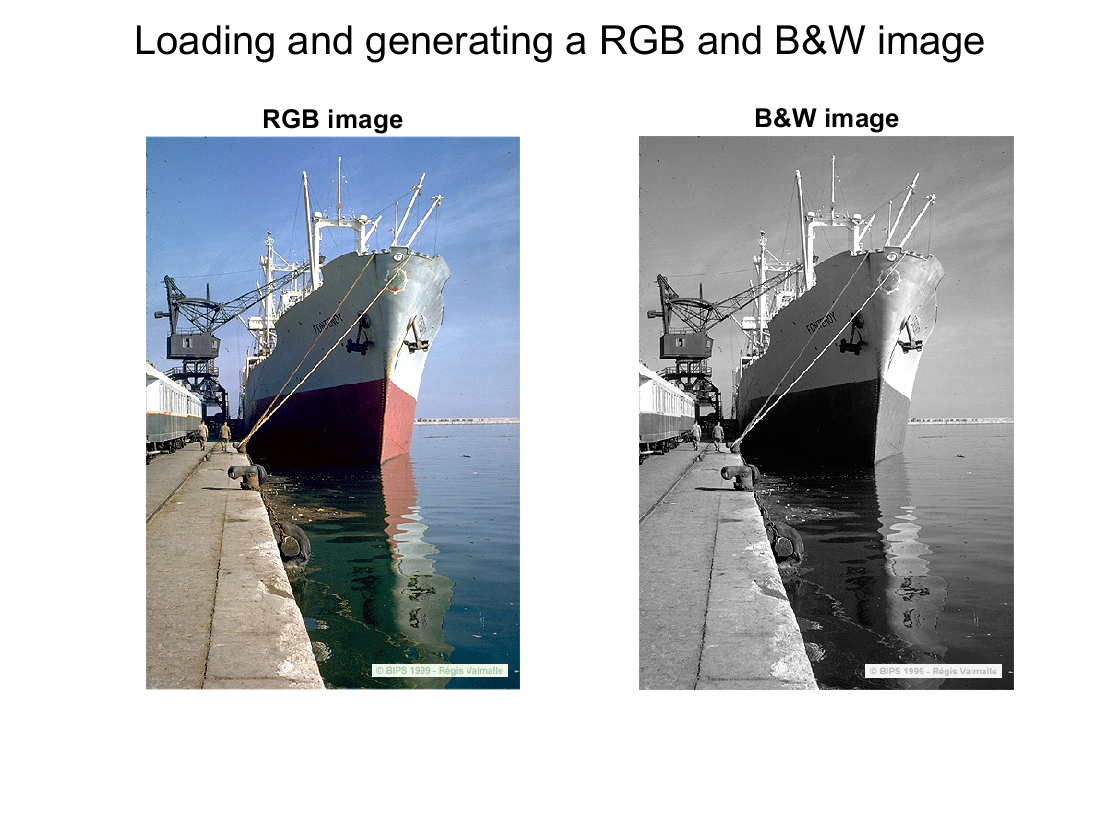
\includegraphics[width=0.5\linewidth]{Doc/Graphics/Part1/Part1_Question1.png}
    \label{fig:enter-label}
\end{figure}


\subsubsection{Greyscale Image Coding}

\textbf{Question 2:}
\textit{Build a matrix with a gradual value of intensity and an horizontal line with a constant value; the representative image is shown Fig. 1.}

\begin{figure}[H]
    \centering
    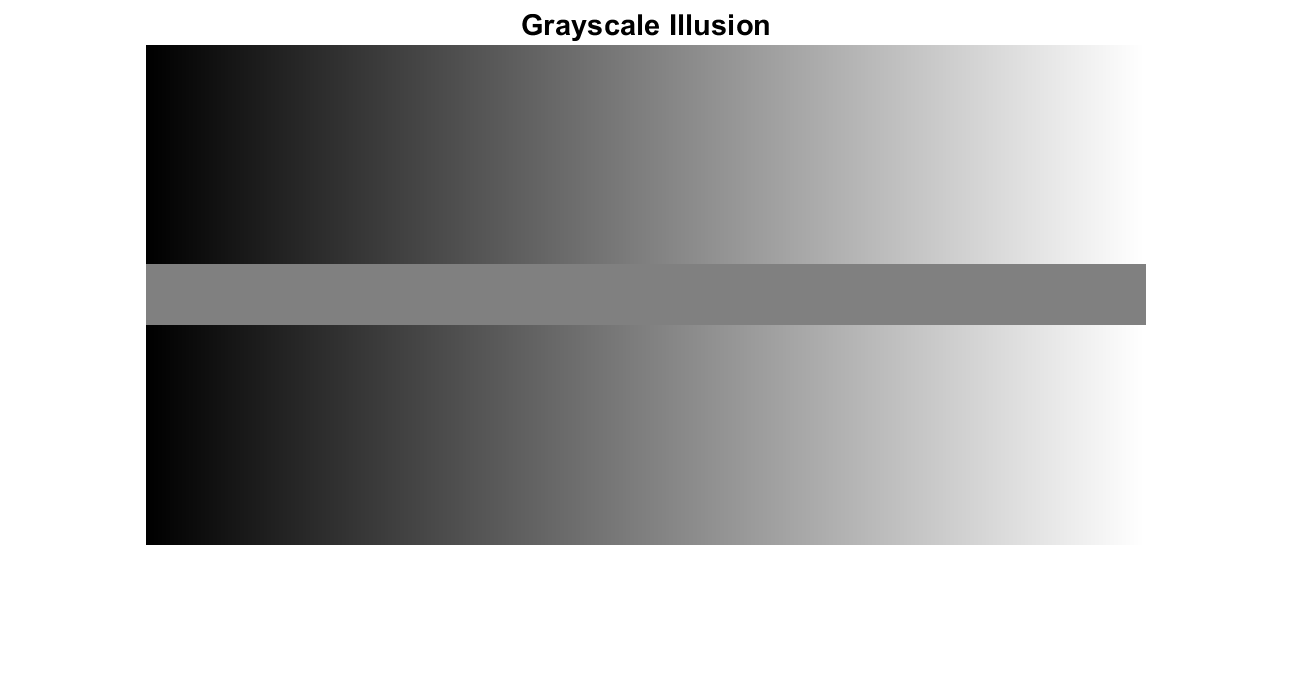
\includegraphics[width=0.5\linewidth]{Doc/Graphics/Part1/Part1_Question2.png}
    \label{fig:enter-label}
\end{figure}



\textbf{Question 3:}
\textit{Build a matrix of black \& white stripes, and with a rectangle and disk as shown Fig. 2. All parameters (size of stripes, size of rectangle, radius) should be easily modifiable.}

\begin{figure}[H]
    \centering
    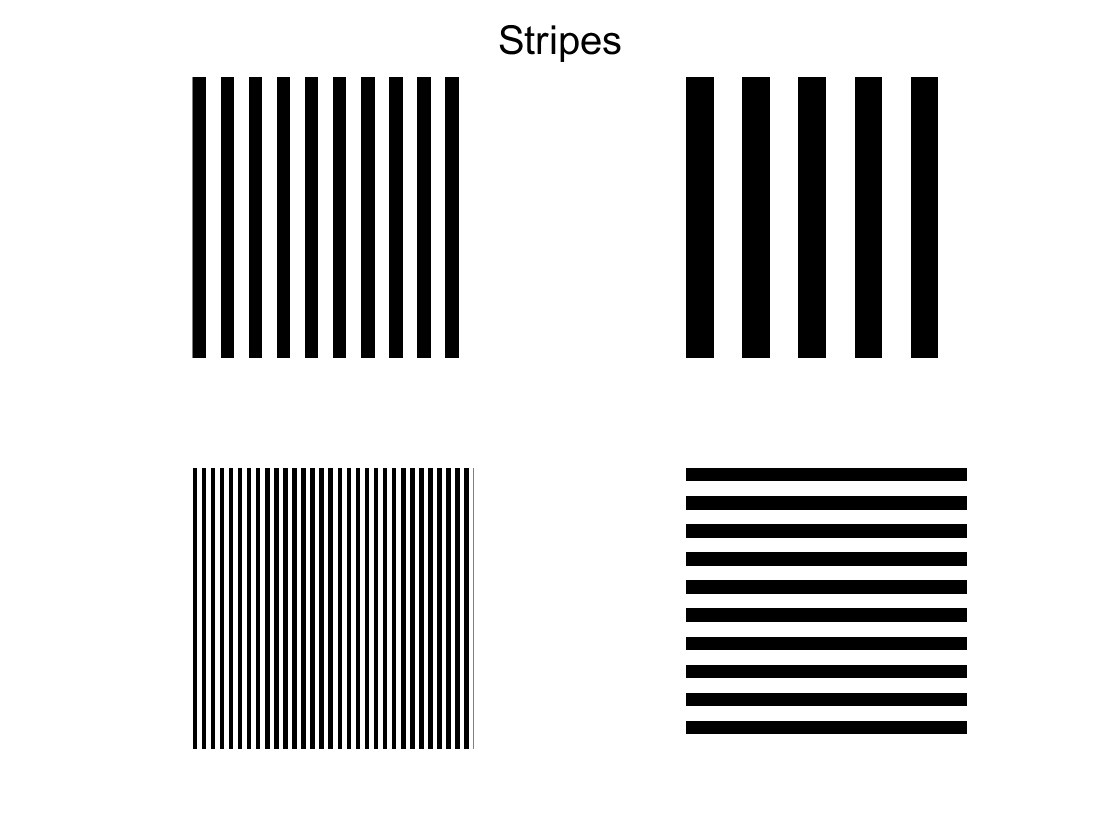
\includegraphics[width=0.75\linewidth]{Doc/Graphics/Part1/Part1_Question3a.png}
    \label{fig:enter-label}
\end{figure}

\begin{figure}[H]
    \centering
    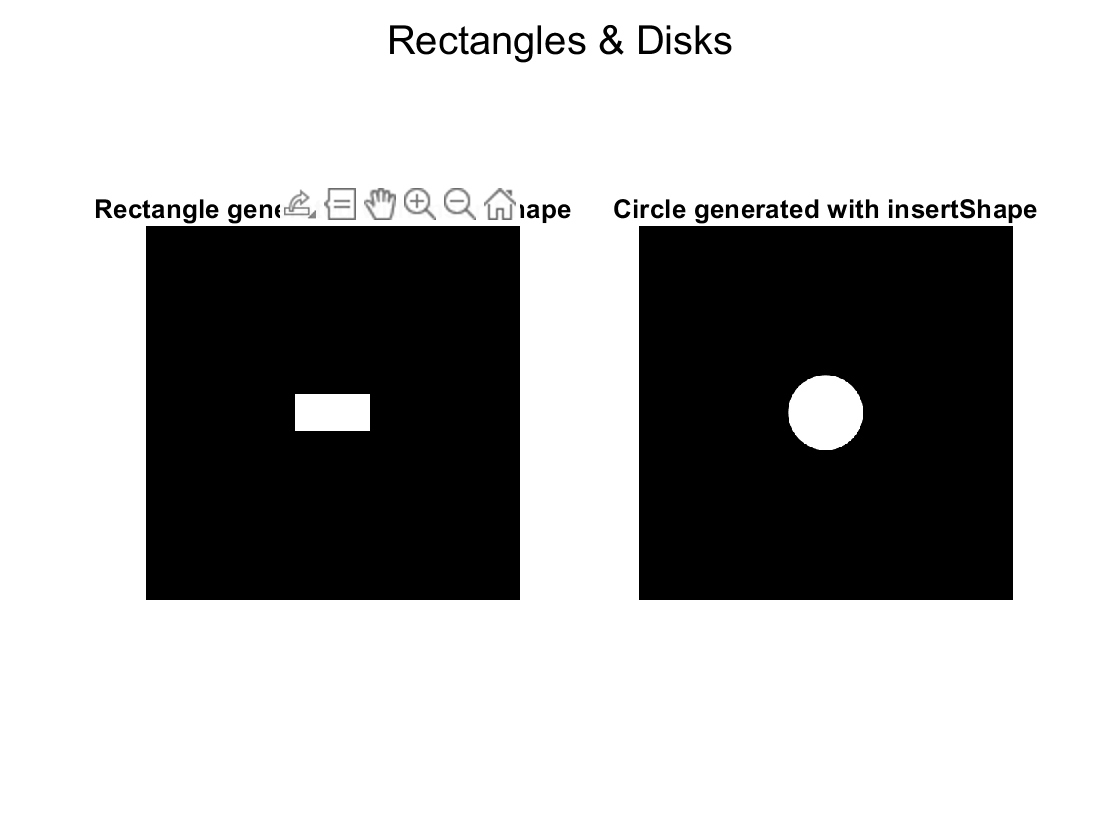
\includegraphics[width=0.5\linewidth]{Doc/Graphics/Part1/Part1_Question3b.png}
    \label{fig:enter-label}
\end{figure}



\subsubsection{Colour Image Coding}
\textbf{Question 4:}
\textit{Next, display Teinte.jpg and its red, green and blue components. Interpret and analyse. Same with oeil.jpg, cargo.jpg and CoulAdd.jpg.}

\begin{figure}[H]
    \centering
    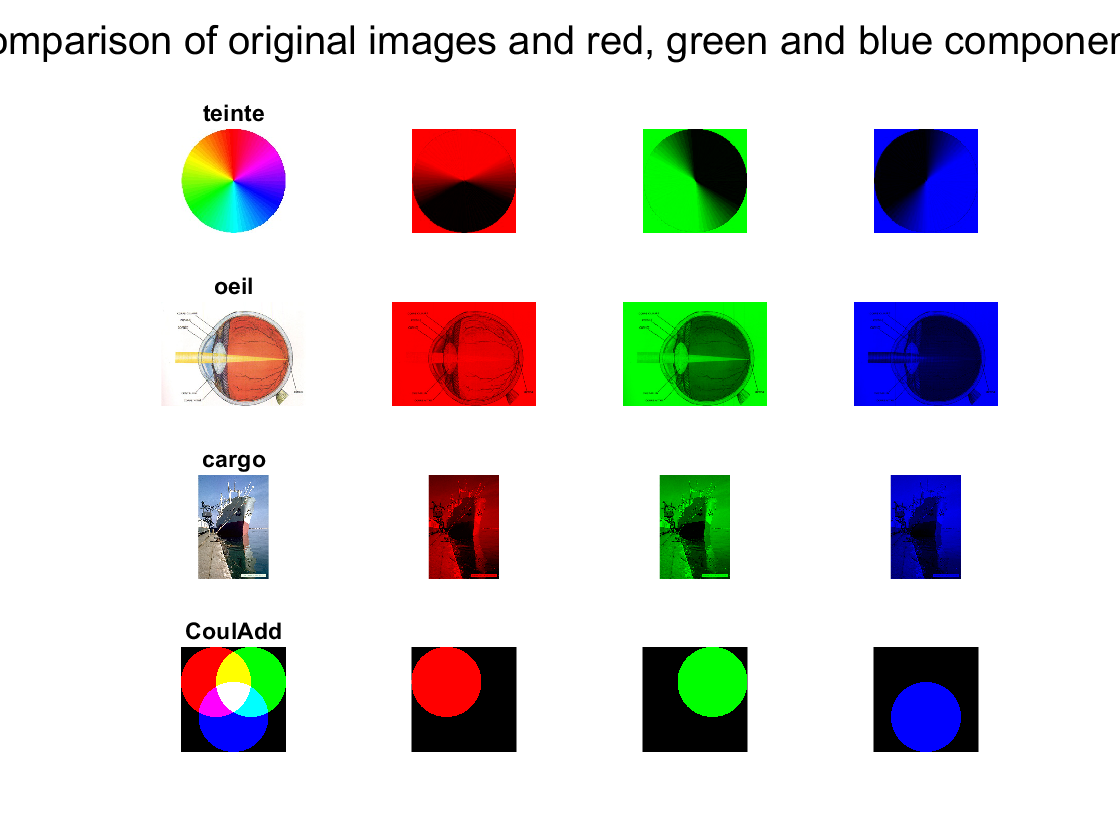
\includegraphics[width=\linewidth]{Doc/Graphics/Part1/Part1_Question4a.png}
    \label{fig:enter-label}
\end{figure}



\textbf{Question 5:}
\textit{Build and display the french flag. Build and display your flag.}

\begin{figure}[H]
    \centering
    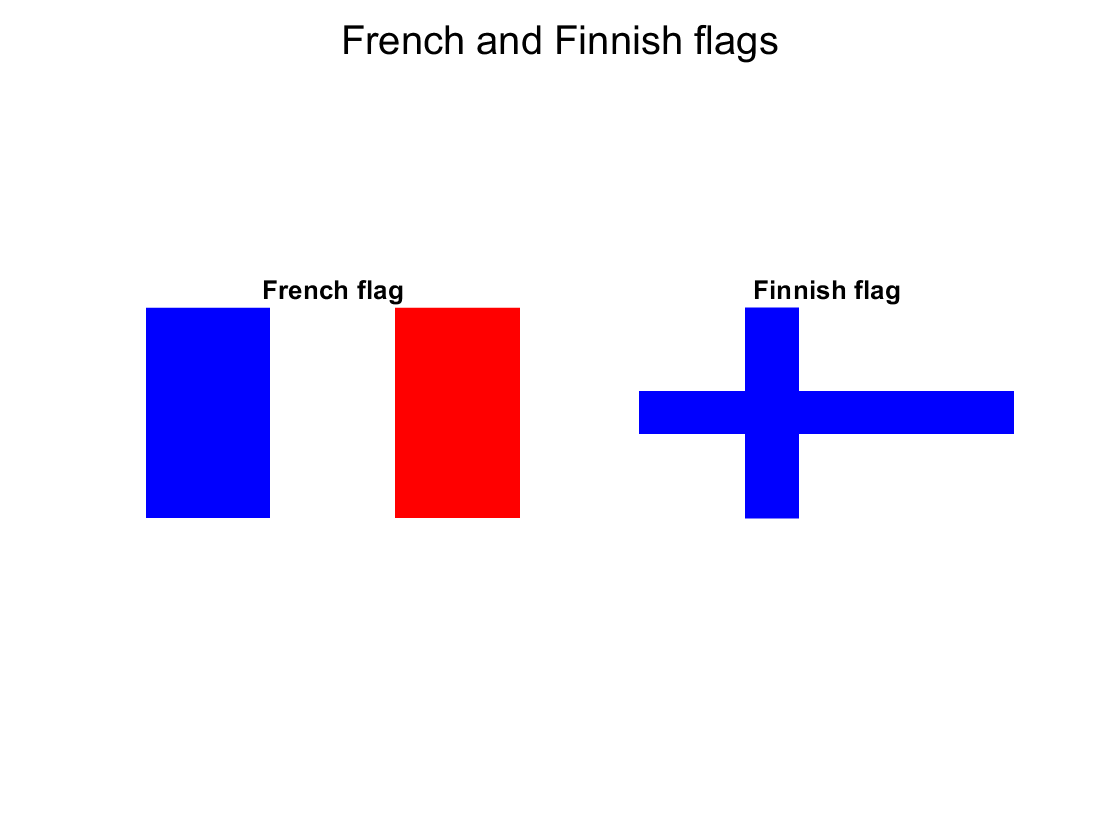
\includegraphics[width=0.5\linewidth]{Doc/Graphics/Part1/Part1_Question5.png}
    \label{fig:enter-label}
\end{figure}


\newpage
\textbf{Question 6:}
\textit{Use the HSV code (with the command rgb2hsv and interpret images. How is the type of the new matrix? Build and display the image Fig. 4.}

\begin{figure}[H]
    \centering
    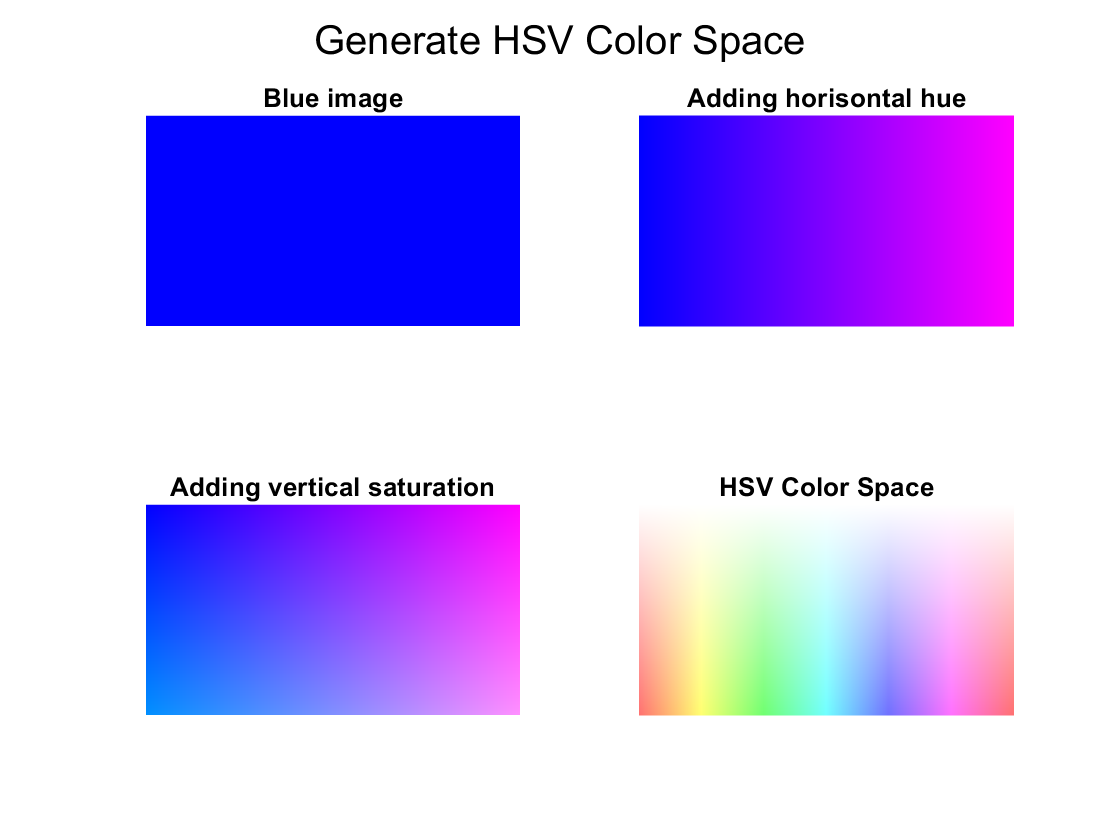
\includegraphics[width=0.75\linewidth]{Doc/Graphics/Part1/Part1_Question6a.png}
    \label{fig:enter-label}
\end{figure}

\begin{figure}[H]
    \centering
    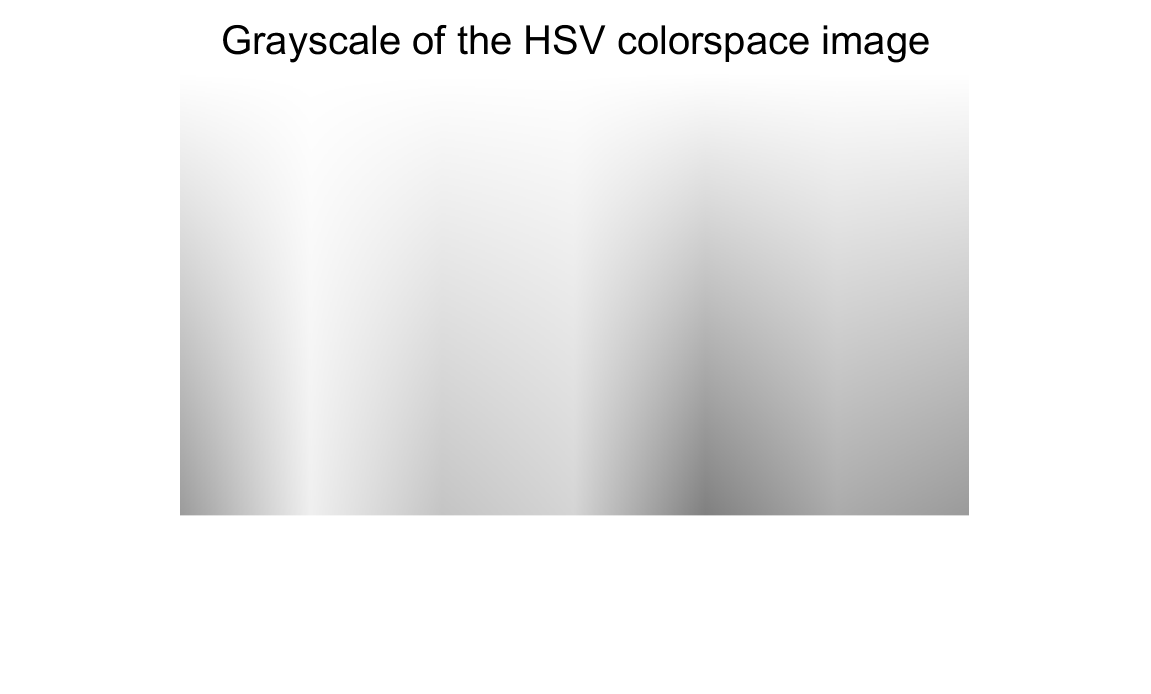
\includegraphics[width=0.5\linewidth]{Doc/Graphics/Part1/Part1_Question6b.png}
    \label{fig:enter-label}
\end{figure}



\textbf{Question 7:}
\textit{What are the values of $\alpha$, $\beta$ and $\gamma$?}

When converting an RGB image to grayscale, the channels get summed according to the weights given by $\alpha$, $\beta$ and $\gamma$:
\begin{equation}
    I = \alpha \cdot r + \beta \cdot g + \gamma \cdot b
\end{equation}
Their values are 
\begin{align*}
    \alpha &= 0.299 \\
    \beta &= 0.587 \\
    \gamma &= 0.114
\end{align*}
to best reflect the way the human vision works, which is much more sensitive to green and red than to blue.

% $\alpha$ and $\beta$ are values used to describe an image's contrast and brightness, respectively. 
% A higher contrast value (>1) increases the difference between pixel values making dark areas darker and bright areas brighter, while a lower value does the opposite. A positive brightness value makes the image brighter by adding intensity, while a negative value makes it darker.
% In a linear transformation of an image, the pixel intensities can be modified with the following equation:
% \[
% I_{\text{new}}(x, y) = \alpha \cdot I_{\text{old}}(x, y) + \beta
% \]

% $\gamma$ correction is a nonlinear transformation applied to an image to adjust both brightness and contrast such that a higher gamma value makes the image darker and a lower value makes it brighter. The formula for gamma correction in the normalised form, i.e., in range [0,1], is:
% \[
% I_{\text{new}}(x, y) = I_{\text{old}}(x, y)^\gamma
% \]

% An example of both forms of correction can be seen in the figure below:

% \begin{figure}[H]
%     \centering
%     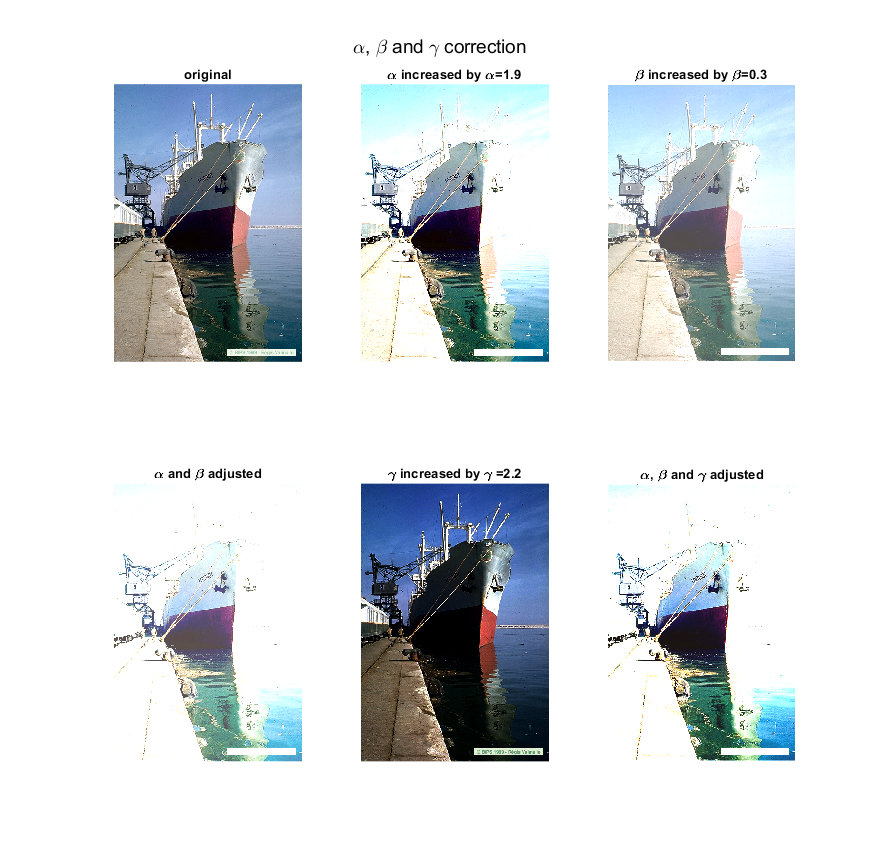
\includegraphics[width=0.6\linewidth]{Doc/Graphics/Part1/Q7.png}
% \end{figure}


\textbf{Question 8:}
\textit{Load and display SpainBeach.png and isolate the beach.}

We can do some primitive feature extraction based on color ranges. While it is difficult to so in RGB as the colors are highly correlated, it is easier to do so in HSV space. We select beach-like colors by selecting a range of hue values, which leads to the result in \autoref{fig:resultQ8}.
\begin{figure}[!ht]
    \centering
    \begin{subfigure}{0.49\textwidth}
        \centering
        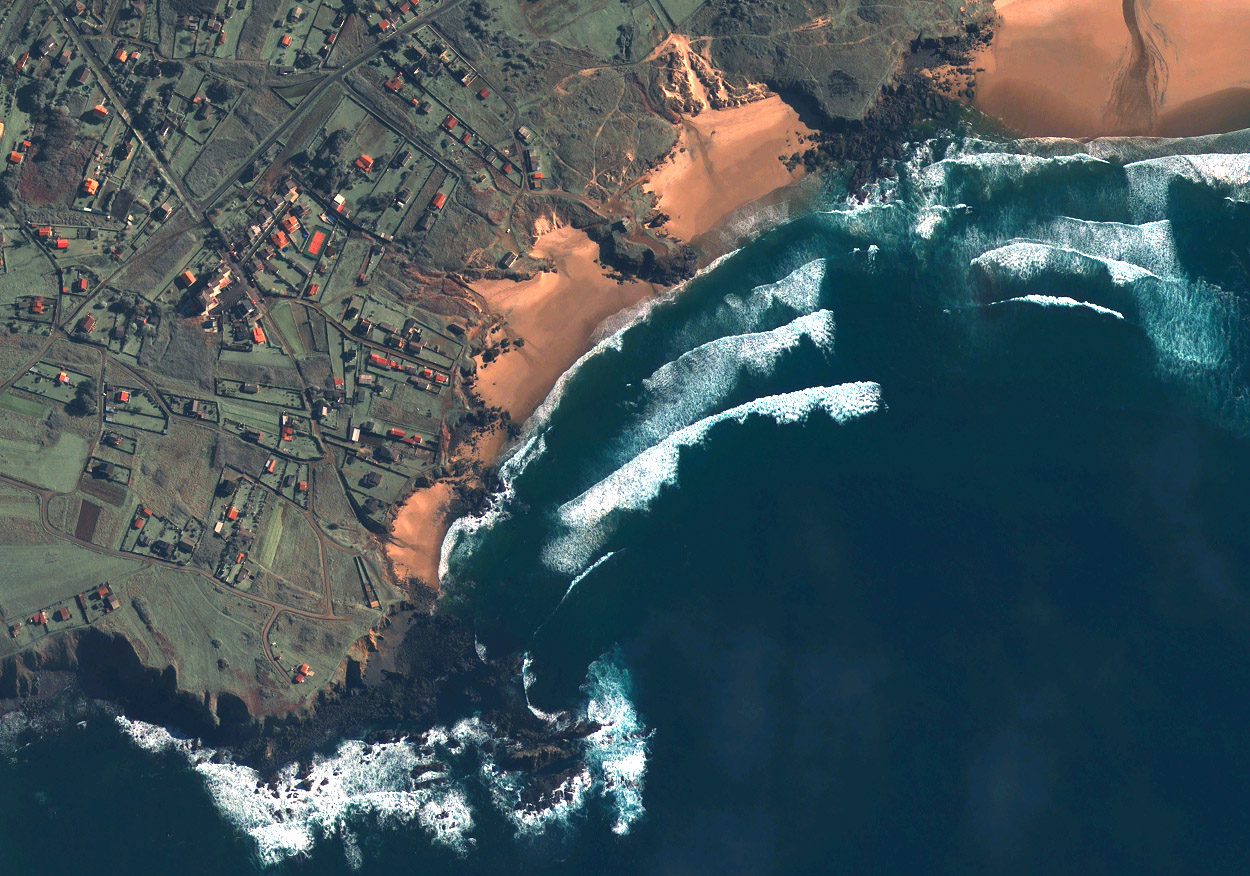
\includegraphics[width=\textwidth]{BE1_IntroComputerVision/SpainBeach.jpg}
        \caption{Original}
    \end{subfigure}
    \hfill
    \begin{subfigure}{0.49\textwidth}
        \centering
        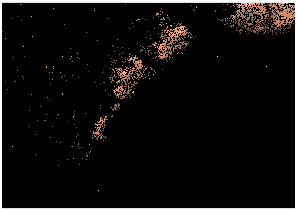
\includegraphics[width=\textwidth]{Doc/Graphics/Part1/Q8_FilteredBeach.png}
        \caption{Filtered beach}
    \end{subfigure}
    \caption{Hue color filtering}
    \label{fig:resultQ8}
\end{figure}


\subsubsection{Histograms}
\textbf{Question 9:}
\textit{What is a histogram? What is the use? Display and interpret histograms of images.}

A histogram of an image represents the intensity level repartition in the image according to the following equation:
\[H_I(n) = \sum_{u} \sum_{v} \{ I(u, v) = n \}\]

However, spatial information is lost. 
If we take the histogram of the Grayscale illusion we can see that the color value in the center bar is clearly overrepresented.
\begin{figure}[!ht]
    \centering
    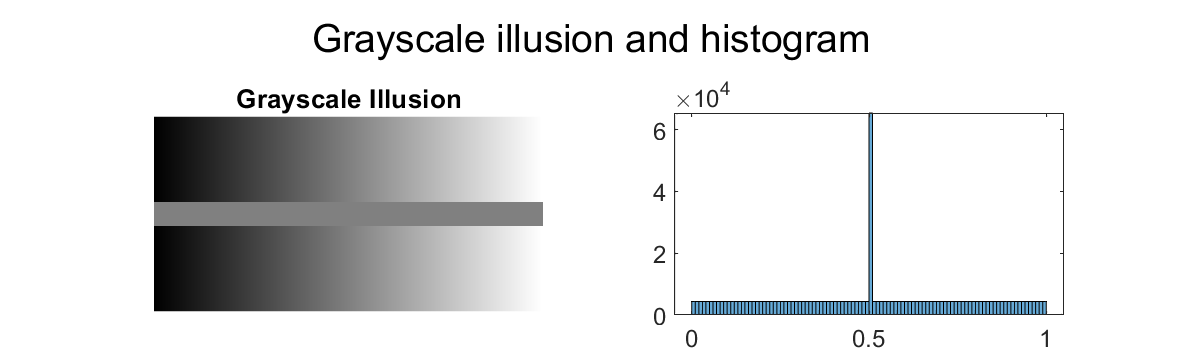
\includegraphics[width=0.75\linewidth]{Doc/Graphics/Part1/part1_Q9.png}
\end{figure}

On the image \texttt{SpainBeach.jpg}, the histogram in \autoref{fig:resultQ9} is less symmetrical. An equalized option is also available, which adjusts the bin size dynamically.
\begin{figure}[!ht]
    \centering
    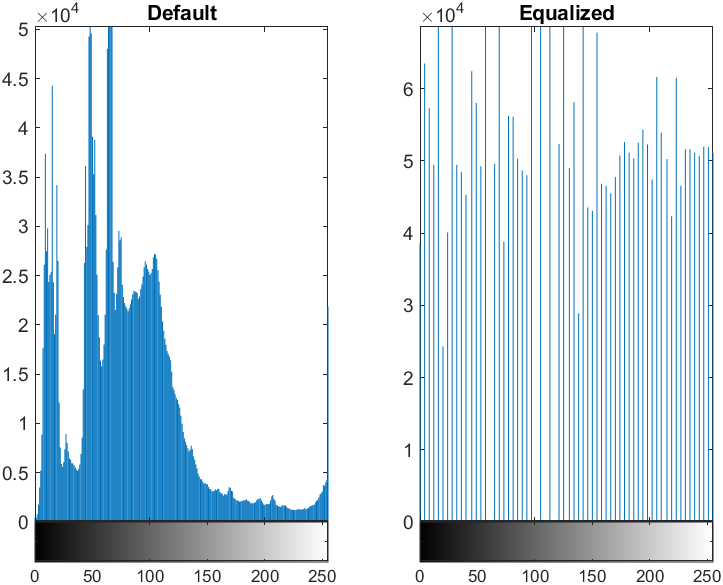
\includegraphics[width=0.5\linewidth]{Doc/Graphics/Part1/Q9_Hist.png}
    \caption{Grayscale histogram}
    \label{fig:resultQ9}
\end{figure}
\FloatBarrier

\textbf{Question 10:}
\textit{Work the mysterious images called Imagex.bmp and Imagexx.bmp.}

Images with the extension \texttt{.bmp} not only include pixel colors, but also a color map. In the case of imagexx this map is empty, leading to a black-looking image by default. However plotting the image as a double data type increases the saturation, and what seems to be the Earth appears, in wrong colors however.
\begin{figure}[!ht]
    \centering
        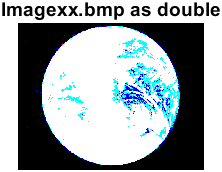
\includegraphics[width=0.5\linewidth]{Doc/Graphics/Part1/Q10_Mystery.png}
    \caption{Mystery image}
    \label{fig:enter-label}
\end{figure}
\FloatBarrier




\subsubsection{Filtering}
\textit{Filtering can be associated to blur and to edge detection. Commands \texttt{imfilter} and \texttt{fspecial} can be used to respectively filter images and define kernel (which can be also defined as a matrix).}


\textbf{Question 11:}
\textit{Apply blur Filtering and Edge filtering on the Stripes images and on a ’real’ image. What are the main associated Kernels ?}

The kernel options for the \texttt{fspecial()} function are:
Average, Disk, Gaussian, Laplacian, Log, Motion, Prewitt, and Sobel. For Edge detection, it is easier to use the \texttt{edge()} function in MatLab, which has the following methods: Sobel, Prewitt, Roberts, Log, Zerocross, Canny and Approxcanny.

The Disk and Motion kernels seem to work best for blurring the stripes images and the Gaussian did not seem to do much. However, the Motion kernel required specific parameters of length and $\theta$ while all tests for other kernels were done with default parameters. The Laplacian and Log kernels seemed to blur everything other than the edges of the stripes, and not even blurring, but not showing anything else just like an edge detection function would. 
The Prewitt and Sobel kernels performed similarly to no surprise as they are edge detection algorithms, however, they did not particularly work for the horizontal stripes.
When applied on a real image, all of these kernels seem to do a decent job at blurring the image. 

For edge detection, the Canny method clearly performs best. For some cases, a combination of the Prewitt and Sobel kernels seemed to perform similarly well, while a combination of the Prewitt and Canny methods gave interesting "green" results.

Different blurring and edge detection kernel- and method options applied on both the stripes image and a real image (\texttt{Champs.jpg})) can be seen in the image below. In particular the Motion kernel for blurring and the Canny and Prewitt methods for edge detection as well as a combination of the two latter methods showing the strange green results.


\begin{figure}[H]
    \centering
    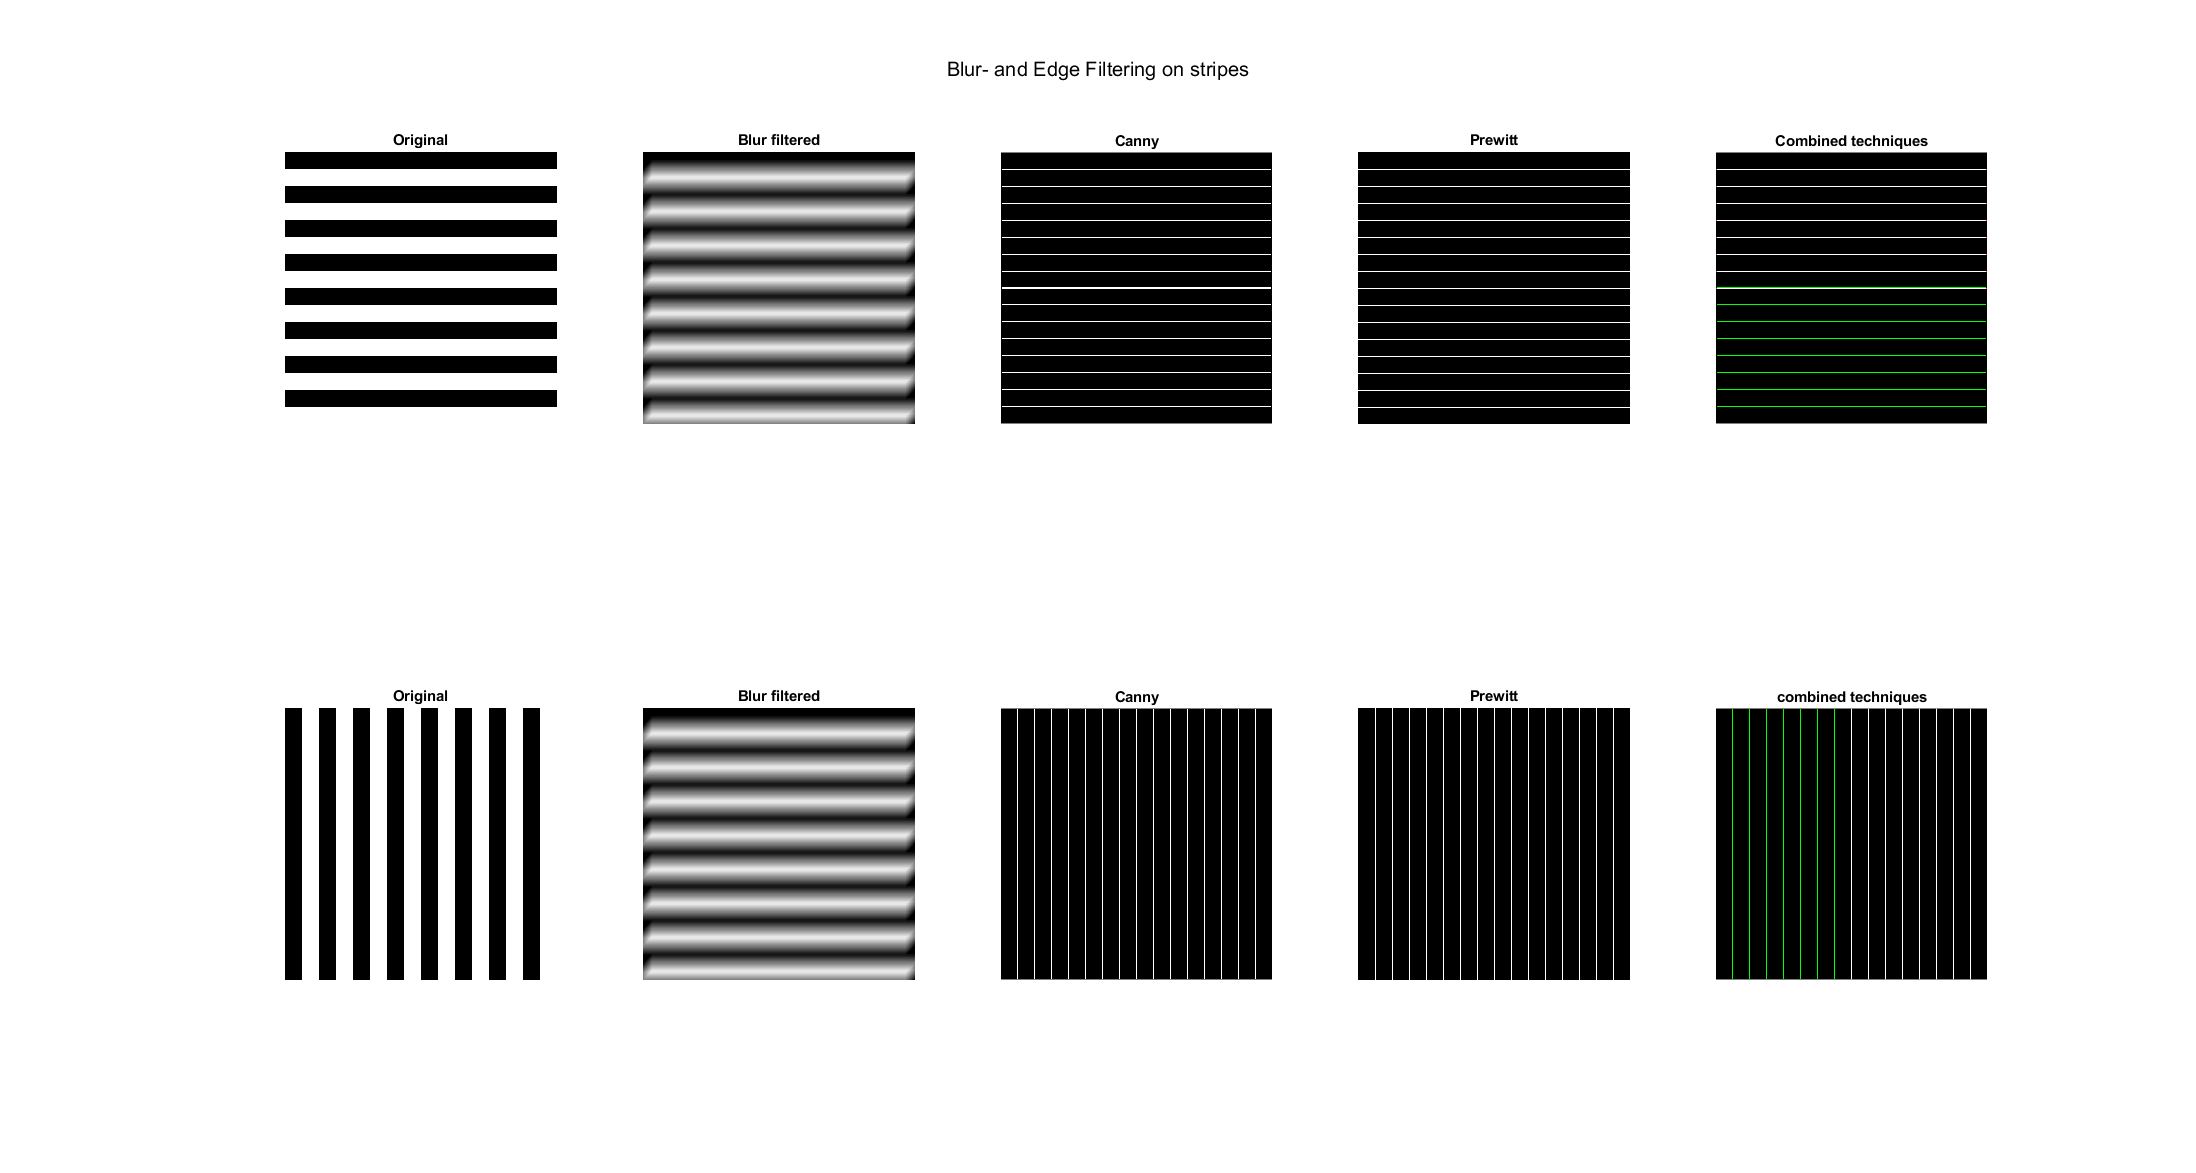
\includegraphics[width=\linewidth]{Doc/Graphics/Part1/Q11a.png}
\end{figure}

\begin{figure}[H]
    \centering
    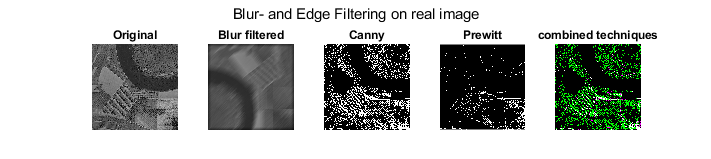
\includegraphics[width=\linewidth]{Doc/Graphics/Part1/Q11b.png}
\end{figure}


\textbf{Question 12:}
\textit{Thanks to successive filtering operators, isolate the main 5 stars of the image Etoiles.png.}

The process to isolate the 5 largest stars can be to first convert the image to grayscale, then smooth the image with a Gaussian filter, then binarise it with an adaptive threshold and finally apply a median filter to remove "salt-and-pepper noise". A comparison was made between a more complicated and simpler approach and the results of the better approaches can be seen below:

\begin{figure}[H]
    \centering
    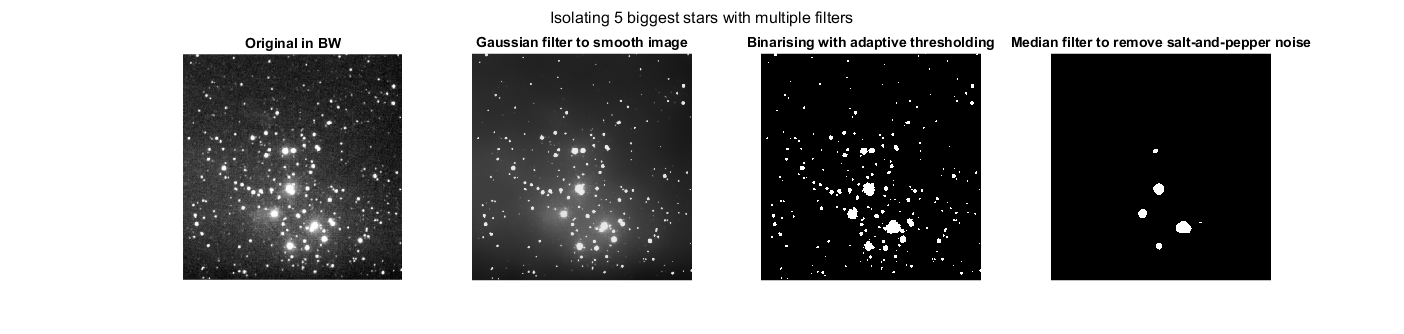
\includegraphics[width=\linewidth]{Doc/Graphics/Part1/Q12a.png}
\end{figure}

\begin{figure}[H]
    \centering
    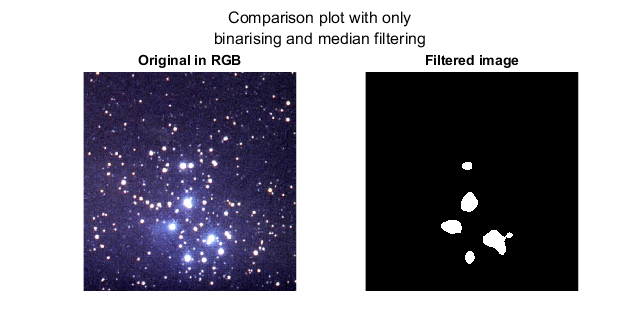
\includegraphics[width=0.5\linewidth]{Doc/Graphics/Part1/Q12b.png}
\end{figure}


\subsection{Fourier Transform}

\textbf{Question 13:}
\textit{Get the FT and analyze the spectrum if images with stripes (Fig. 2), rectangle and disks (Fig. 3).}

The Fourier transform seems to exhibit a repeating pattern that is close to the original shape, such as the concentric circles and the rectangles. As a rule of thumb the orientation of the periodic features, such as the stripes can also be found in the spectrum again.

\begin{figure}[!ht]
    \centering
    \begin{subfigure}{0.32\textwidth}
        \centering
        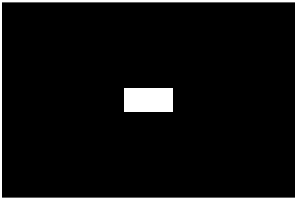
\includegraphics[width=\textwidth]{Doc/Graphics/Part1/Q3_rect.png}
        \caption{Original}
    \end{subfigure}
    \hfill
    \begin{subfigure}{0.32\textwidth}
        \centering
        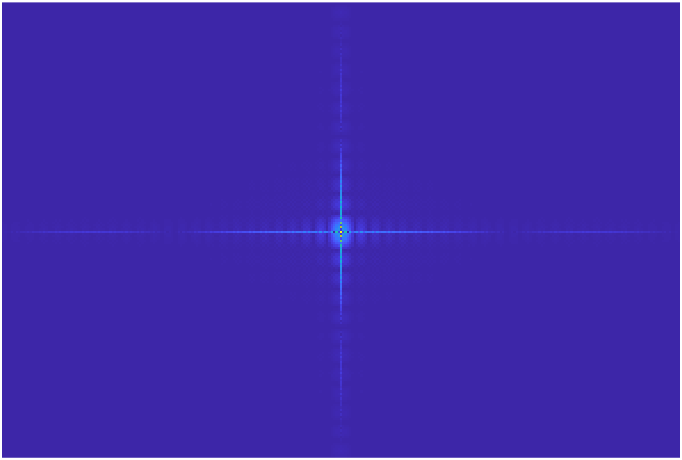
\includegraphics[width=\textwidth]{Doc/Graphics/Part1/Q13_Rectangle.png}
        \caption{Linear Spectrum}
    \end{subfigure}
    \hfill
    \begin{subfigure}{0.32\textwidth}
        \centering
        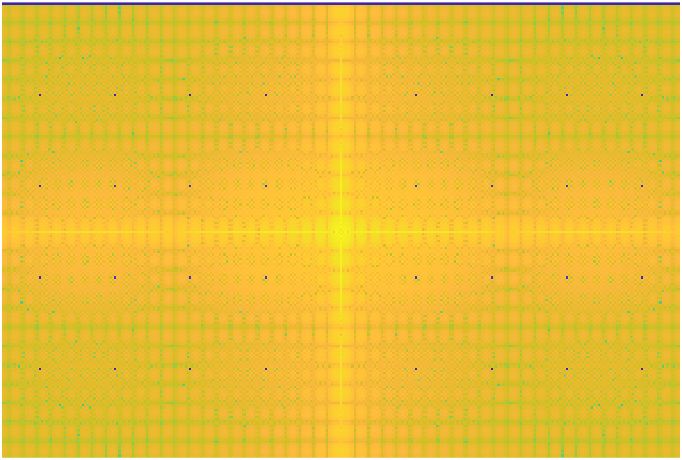
\includegraphics[width=\textwidth]{Doc/Graphics/Part1/Q13_log_Rectangle.png}
        \caption{Log Spectrum}
    \end{subfigure}
    \caption{Fourier transform of rectangle}
\end{figure}

\begin{figure}[!ht]
    \centering
    \begin{subfigure}{0.32\textwidth}
        \centering
        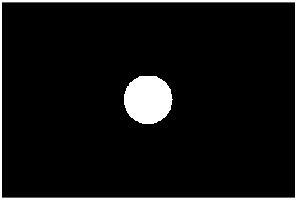
\includegraphics[width=\textwidth]{Doc/Graphics/Part1/Q3_circ.png}
        \caption{Original}
    \end{subfigure}
    \hfill
    \begin{subfigure}{0.32\textwidth}
        \centering
        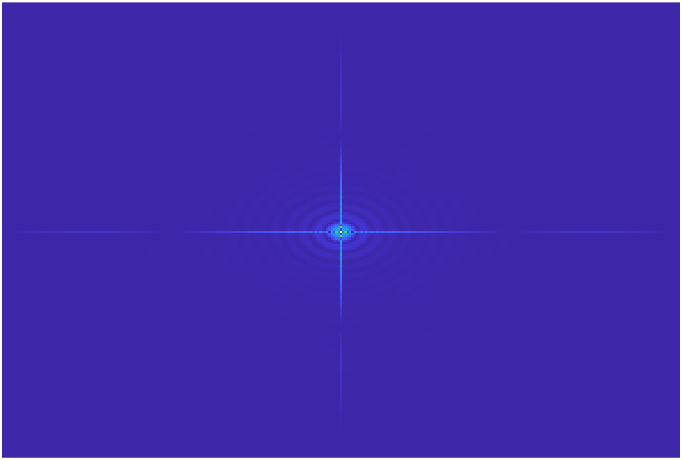
\includegraphics[width=\textwidth]{Doc/Graphics/Part1/Q13_Circle.png}
        \caption{Linear Spectrum}
    \end{subfigure}
    \hfill
    \begin{subfigure}{0.32\textwidth}
        \centering
        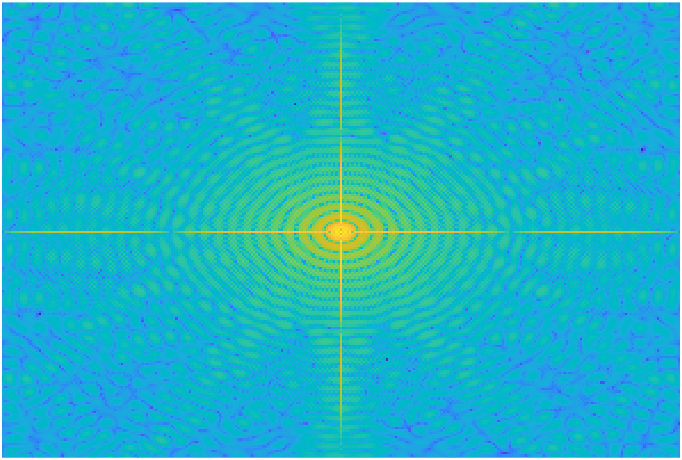
\includegraphics[width=\textwidth]{Doc/Graphics/Part1/Q13_log_Circle.png}
        \caption{Log Spectrum}
    \end{subfigure}
    \caption{Fourier transform of circle}
\end{figure}
\begin{figure}[!ht]
    \centering
    \begin{subfigure}{0.32\textwidth}
        \centering
        
\includegraphics[width=\textwidth]{Doc/Graphics/Part1/Q3_hstripes.png}
        \caption{Original}
    \end{subfigure}
    \hfill
    \begin{subfigure}{0.32\textwidth}
        \centering
        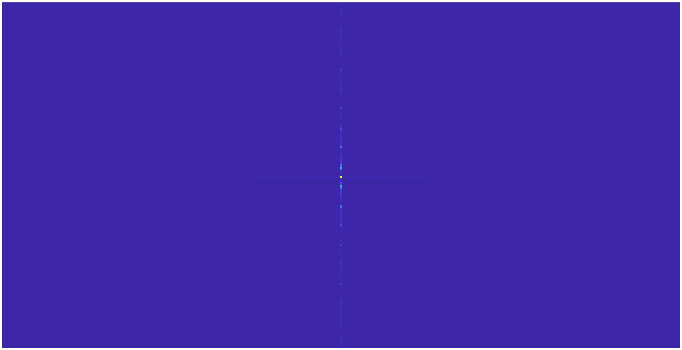
\includegraphics[width=\textwidth]{Doc/Graphics/Part1/Q13_Horizontal stripes.png}
        \caption{Linear Spectrum}
    \end{subfigure}
    \hfill
    \begin{subfigure}{0.32\textwidth}
        \centering
        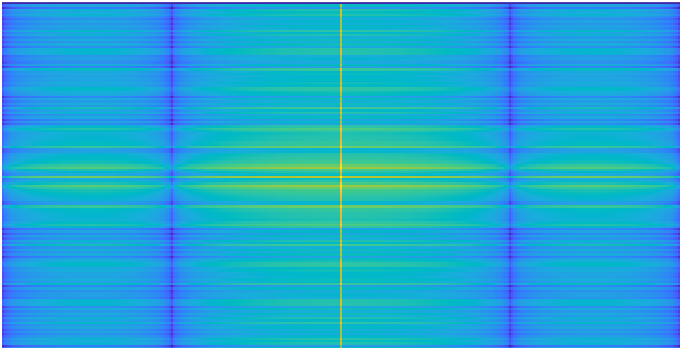
\includegraphics[width=\textwidth]{Doc/Graphics/Part1/Q13_log_Horizontal stripes.png}
        \caption{Log Spectrum}
    \end{subfigure}
    \caption{Fourier transform of horizontal stripes}
\end{figure}
\begin{figure}[!ht]
    \centering
    \begin{subfigure}{0.32\textwidth}
        \centering
        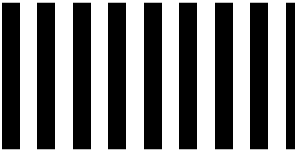
\includegraphics[width=\textwidth]{Doc/Graphics/Part1/Q3_vstripes.png}
        \caption{Original}
    \end{subfigure}
    \hfill
    \begin{subfigure}{0.32\textwidth}
        \centering
        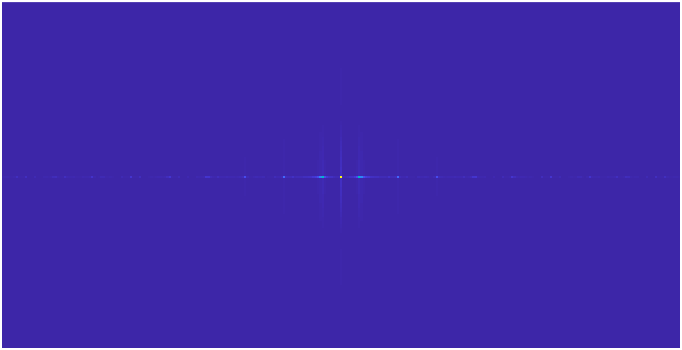
\includegraphics[width=\textwidth]{Doc/Graphics/Part1/Q13_Vertical stripes.png}
        \caption{Linear Spectrum}
    \end{subfigure}
    \hfill
    \begin{subfigure}{0.32\textwidth}
        \centering
        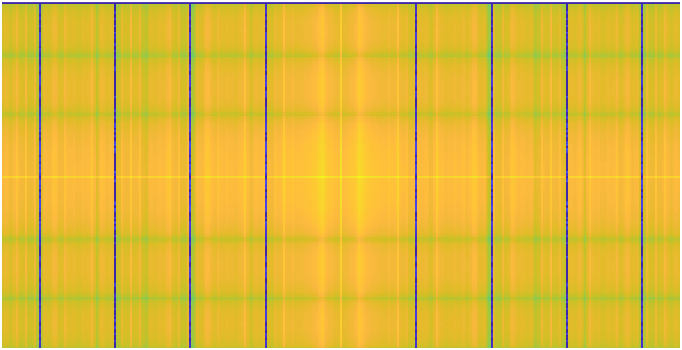
\includegraphics[width=\textwidth]{Doc/Graphics/Part1/Q13_log_Vertical stripes.png}
        \caption{Log Spectrum}
    \end{subfigure}
    \caption{Fourier transform of vertical stripes}
\end{figure}
\FloatBarrier

% \begin{figure}[H]
%     \centering
%     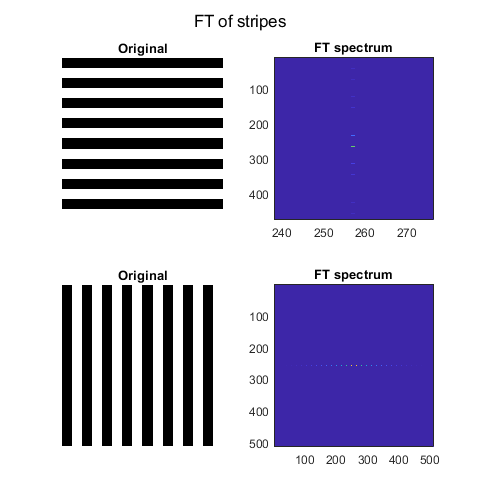
\includegraphics[width=0.75\linewidth]{Doc/Graphics/Part1/part1_Question13b.png}
% \end{figure}

% \begin{figure}[H]
%     \centering
%     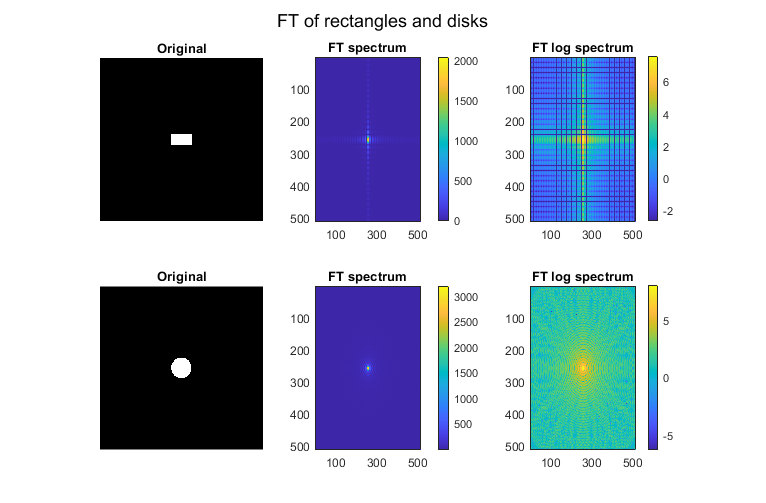
\includegraphics[width=\linewidth]{Doc/Graphics/Part1/Part1_Question13a.png}
% \end{figure}




\textbf{Question 14:}
\textit{Blur the image with different kernels and interpret the spectrum.}

As we blur the images with larger disks, the blur is more pronounced. In the Fourier transform spectrum this results in high frequencies getting eliminated and the low frequencies around the origin becoming more pronounced. This is to be expected, as blurring eliminates small details which yield high frequencies in the spectrum. 

At the same time, the blurred spectra also show that similar features to both the image and the blurring kernel. In this case, we blur the image with a disk, which leads to the emergence of circular patterns in the spectrum. This can be lead back to the mathematical relation that a convolution is equal to a multiplication in the frequency domain.

\begin{figure}[!ht]
    \centering
    \begin{subfigure}{0.24\textwidth}
        \centering
        \adjustbox{valign=c}{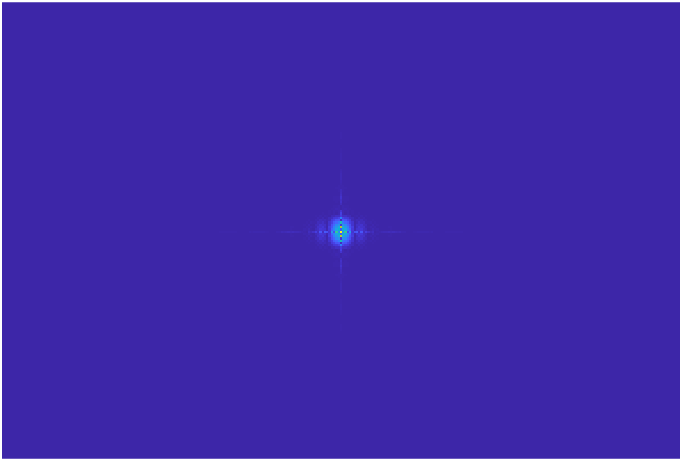
\includegraphics[width=\textwidth]{Doc/Graphics/Part1/Q14_Disk10_Rectangle.png}}
    \end{subfigure}
    \hfill
    \begin{subfigure}{0.24\textwidth}
        \centering
        \adjustbox{valign=c}{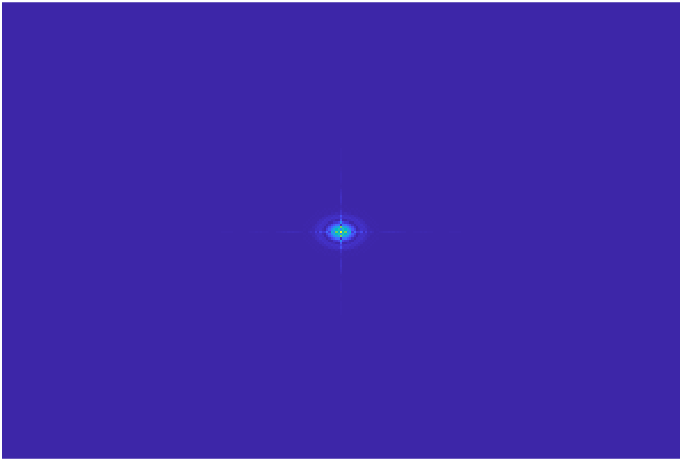
\includegraphics[width=\textwidth]{Doc/Graphics/Part1/Q14_Disk10_Circle.png}}
    \end{subfigure}
    \hfill
    \begin{subfigure}{0.24\textwidth}
        \centering
        \adjustbox{valign=c}{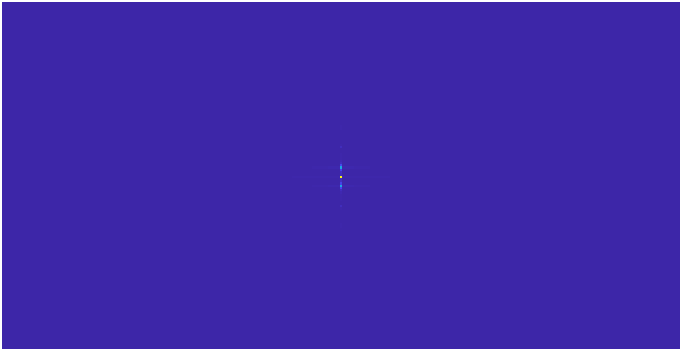
\includegraphics[width=\textwidth]{Doc/Graphics/Part1/Q14_Disk10_Horizontal stripes.png}}
    \end{subfigure}
    \hfill
    \begin{subfigure}{0.24\textwidth}
        \centering
        \adjustbox{valign=c}{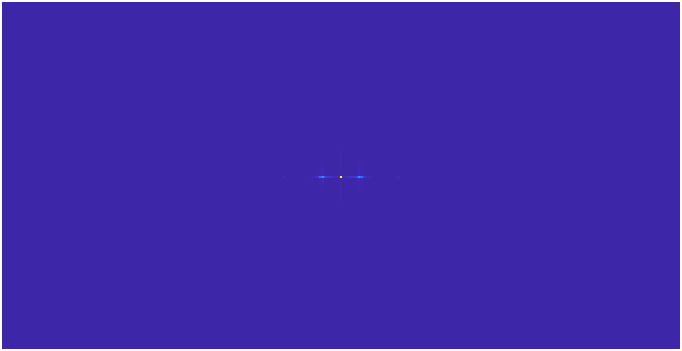
\includegraphics[width=\textwidth]{Doc/Graphics/Part1/Q14_Disk10_Vertical stripes.png}}
    \end{subfigure}

    \begin{subfigure}{0.24\textwidth}
        \centering
        \adjustbox{valign=c}{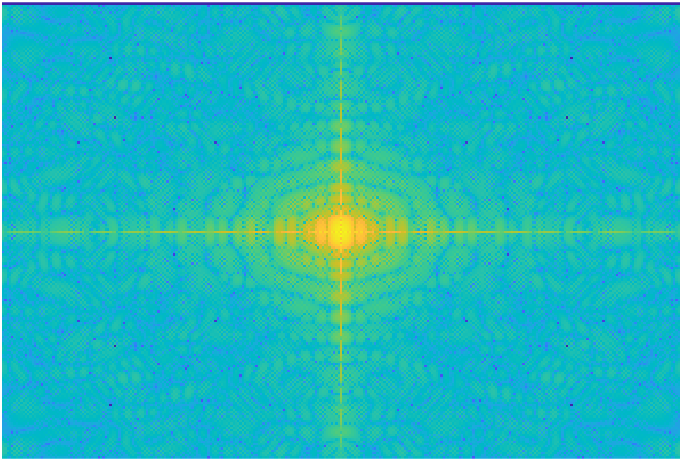
\includegraphics[width=\textwidth]{Doc/Graphics/Part1/Q14_Disk10_log_Rectangle.png}}
    \end{subfigure}
    \hfill
    \begin{subfigure}{0.24\textwidth}
        \centering
        \adjustbox{valign=c}{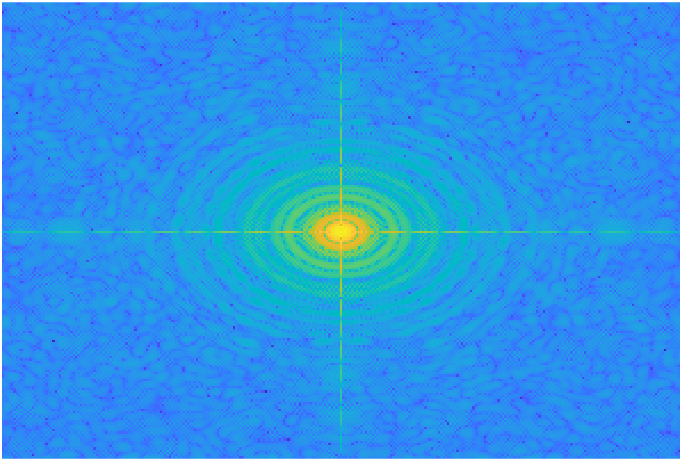
\includegraphics[width=\textwidth]{Doc/Graphics/Part1/Q14_Disk10_log_Circle.png}}
    \end{subfigure}
    \hfill
    \begin{subfigure}{0.24\textwidth}
        \centering
        \adjustbox{valign=c}{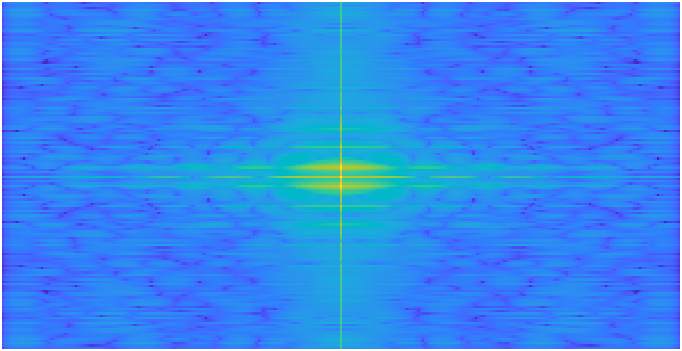
\includegraphics[width=\textwidth]{Doc/Graphics/Part1/Q14_Disk10_log_Horizontal stripes.png}}
    \end{subfigure}
    \hfill
    \begin{subfigure}{0.24\textwidth}
        \centering
        \adjustbox{valign=c}{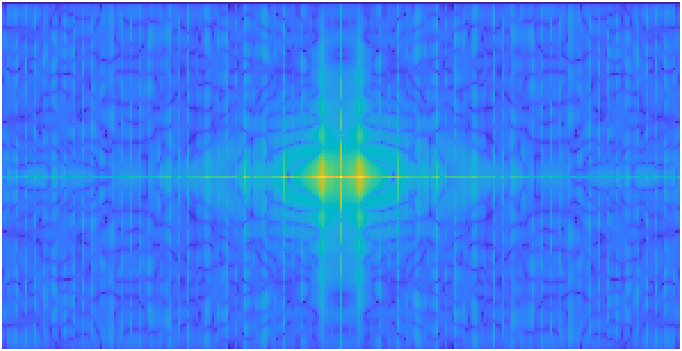
\includegraphics[width=\textwidth]{Doc/Graphics/Part1/Q14_Disk10_log_Vertical stripes.png}}
    \end{subfigure}
    \caption{Blurring with disk of radius 10}
    \label{fig:resultQ14Disk10}
\end{figure}

\begin{figure}[!ht]
    \centering
    \begin{subfigure}{0.24\textwidth}
        \centering
        \adjustbox{valign=c}{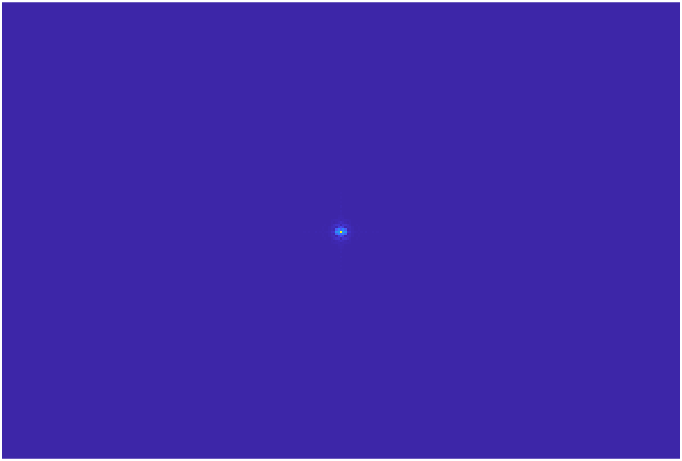
\includegraphics[width=\textwidth]{Doc/Graphics/Part1/Q14_Disk50_Rectangle.png}}
    \end{subfigure}
    \hfill
    \begin{subfigure}{0.24\textwidth}
        \centering
        \adjustbox{valign=c}{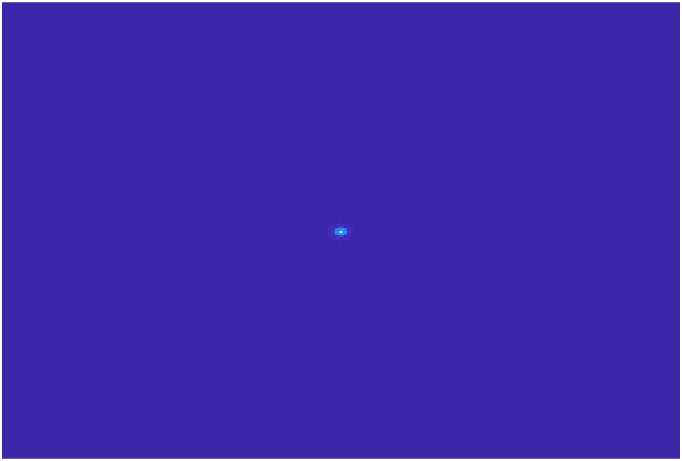
\includegraphics[width=\textwidth]{Doc/Graphics/Part1/Q14_Disk50_Circle.png}}
    \end{subfigure}
    \hfill
    \begin{subfigure}{0.24\textwidth}
        \centering
        \adjustbox{valign=c}{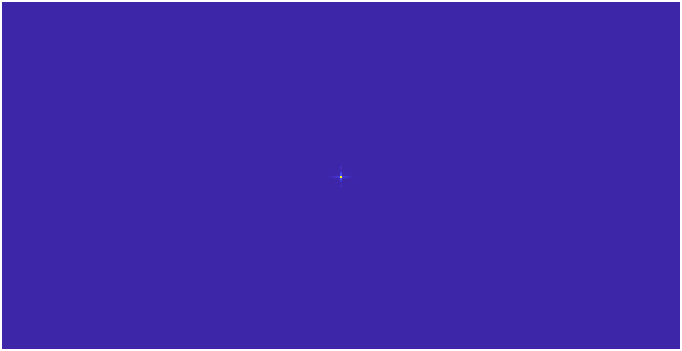
\includegraphics[width=\textwidth]{Doc/Graphics/Part1/Q14_Disk50_Horizontal stripes.png}}
    \end{subfigure}
    \hfill
    \begin{subfigure}{0.24\textwidth}
        \centering
        \adjustbox{valign=c}{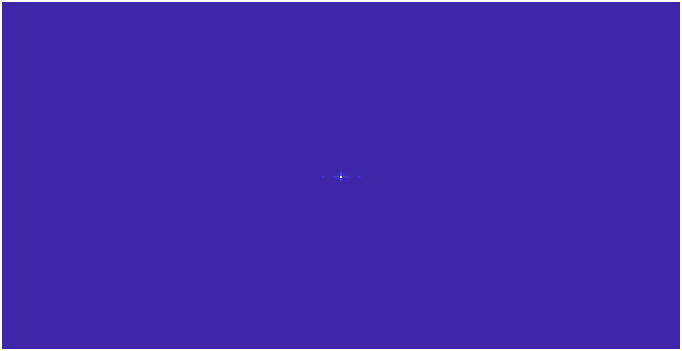
\includegraphics[width=\textwidth]{Doc/Graphics/Part1/Q14_Disk50_Vertical stripes.png}}
    \end{subfigure}
    
    \begin{subfigure}{0.24\textwidth}
        \centering
        \adjustbox{valign=c}{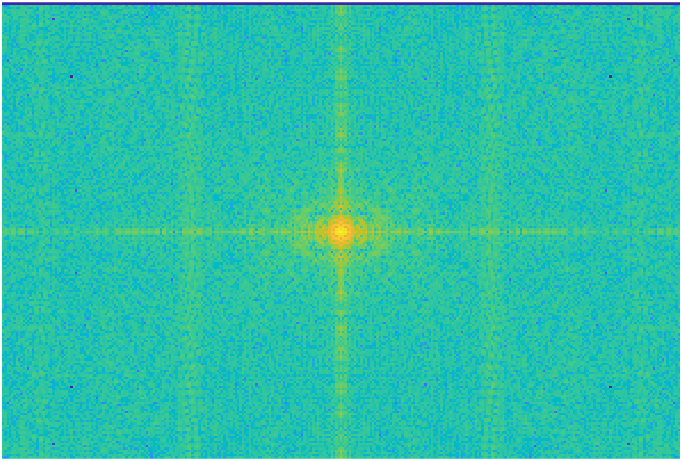
\includegraphics[width=\textwidth]{Doc/Graphics/Part1/Q14_Disk50_log_Rectangle.png}}
    \end{subfigure}
    \hfill
    \begin{subfigure}{0.24\textwidth}
        \centering
        \adjustbox{valign=c}{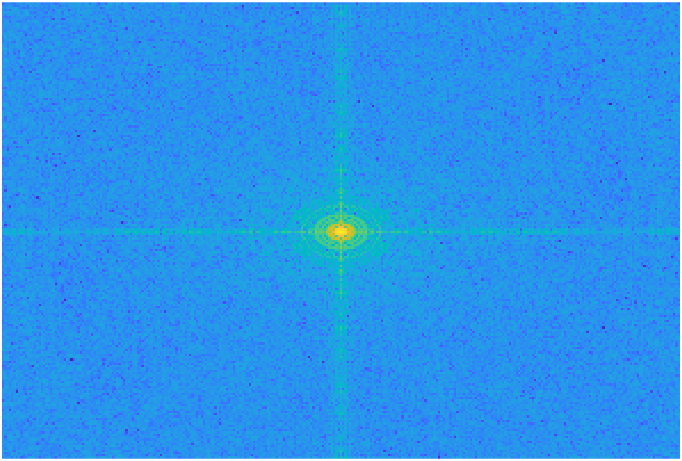
\includegraphics[width=\textwidth]{Doc/Graphics/Part1/Q14_Disk50_log_Circle.png}}
    \end{subfigure}
    \hfill
    \begin{subfigure}{0.24\textwidth}
        \centering
        \adjustbox{valign=c}{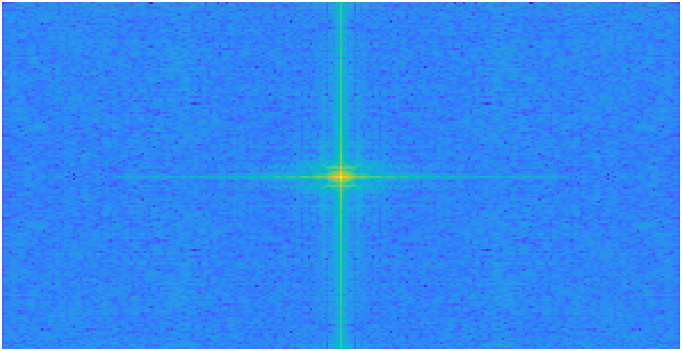
\includegraphics[width=\textwidth]{Doc/Graphics/Part1/Q14_Disk50_log_Horizontal stripes.png}}
    \end{subfigure}
    \hfill
    \begin{subfigure}{0.24\textwidth}
        \centering
        \adjustbox{valign=c}{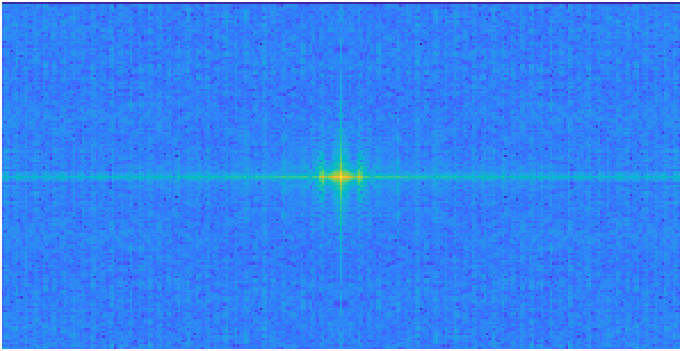
\includegraphics[width=\textwidth]{Doc/Graphics/Part1/Q14_Disk50_log_Vertical stripes.png}}
    \end{subfigure}
    \caption{Blurring with disk of radius 50}
    \label{fig:resultQ14Disk50}
\end{figure}
\FloatBarrier


% \textbf{Stripes:}
% An analysis of the different blurring kernel option performances can be seen in the answer for \textit{Question 12. The FT on the other hand...}

% \begin{figure}[H]
%     \centering
%     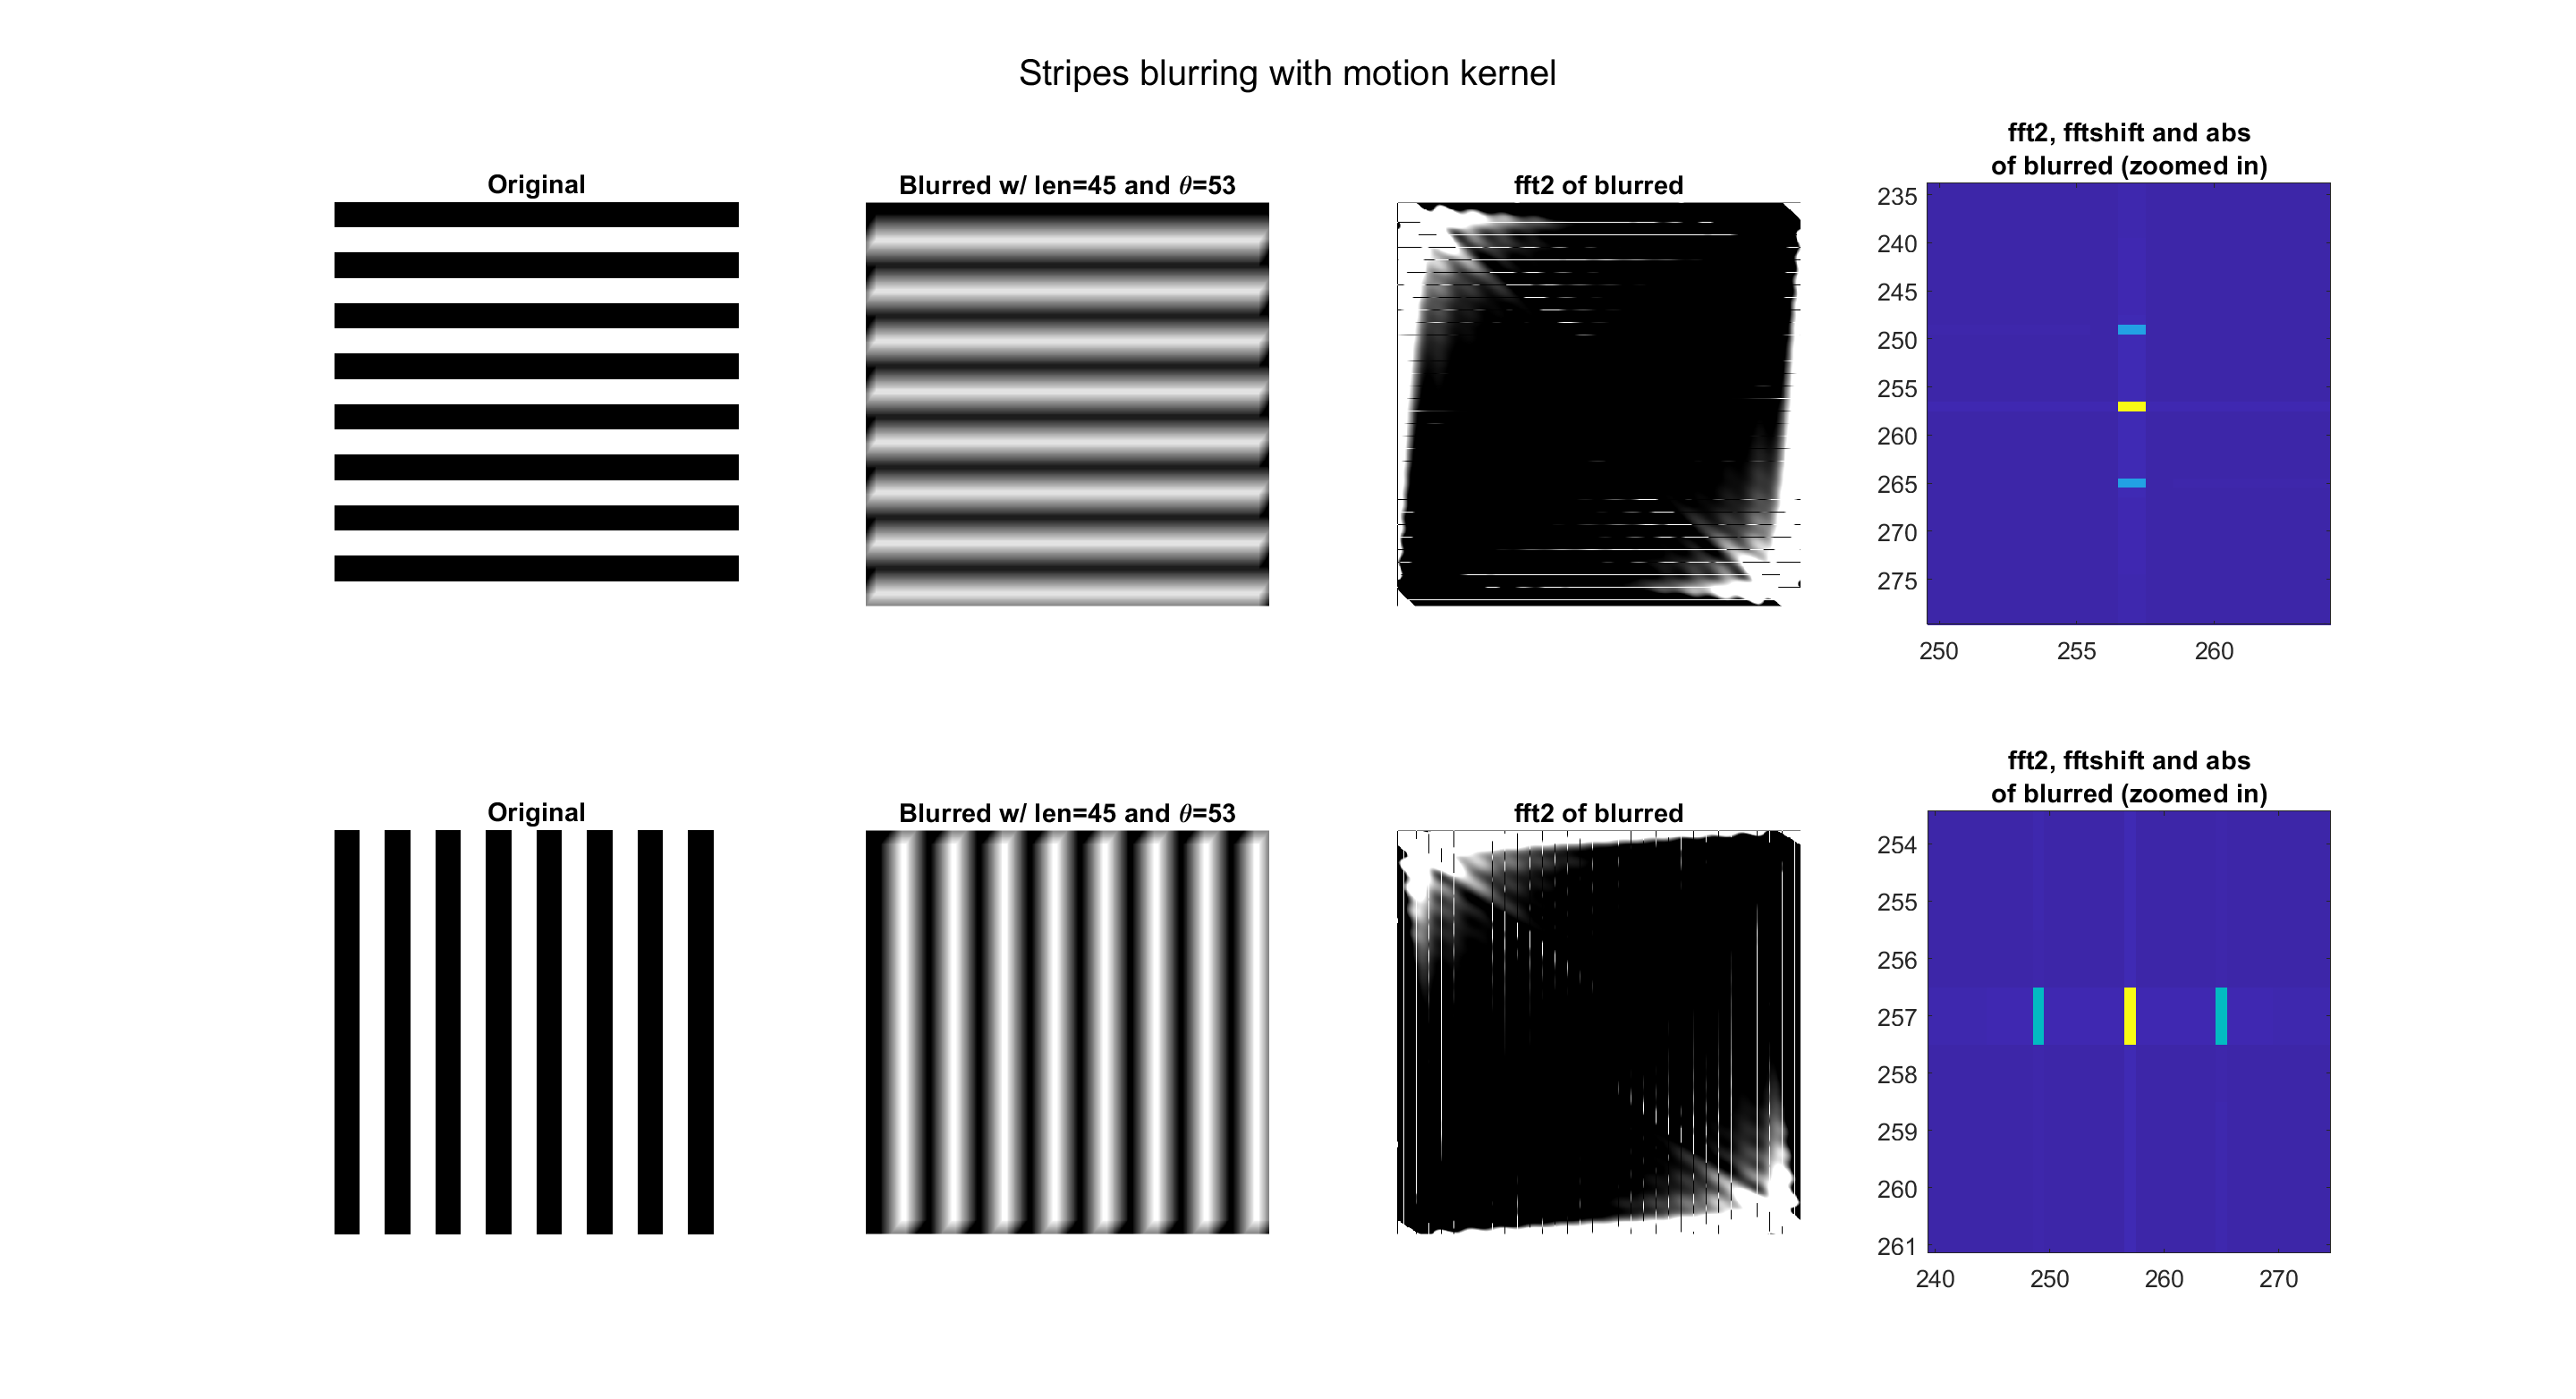
\includegraphics[width=0.75\linewidth]{Doc/Graphics/Part1/Q14a.png}
% \end{figure}

% \begin{figure}[H]
%     \centering
%     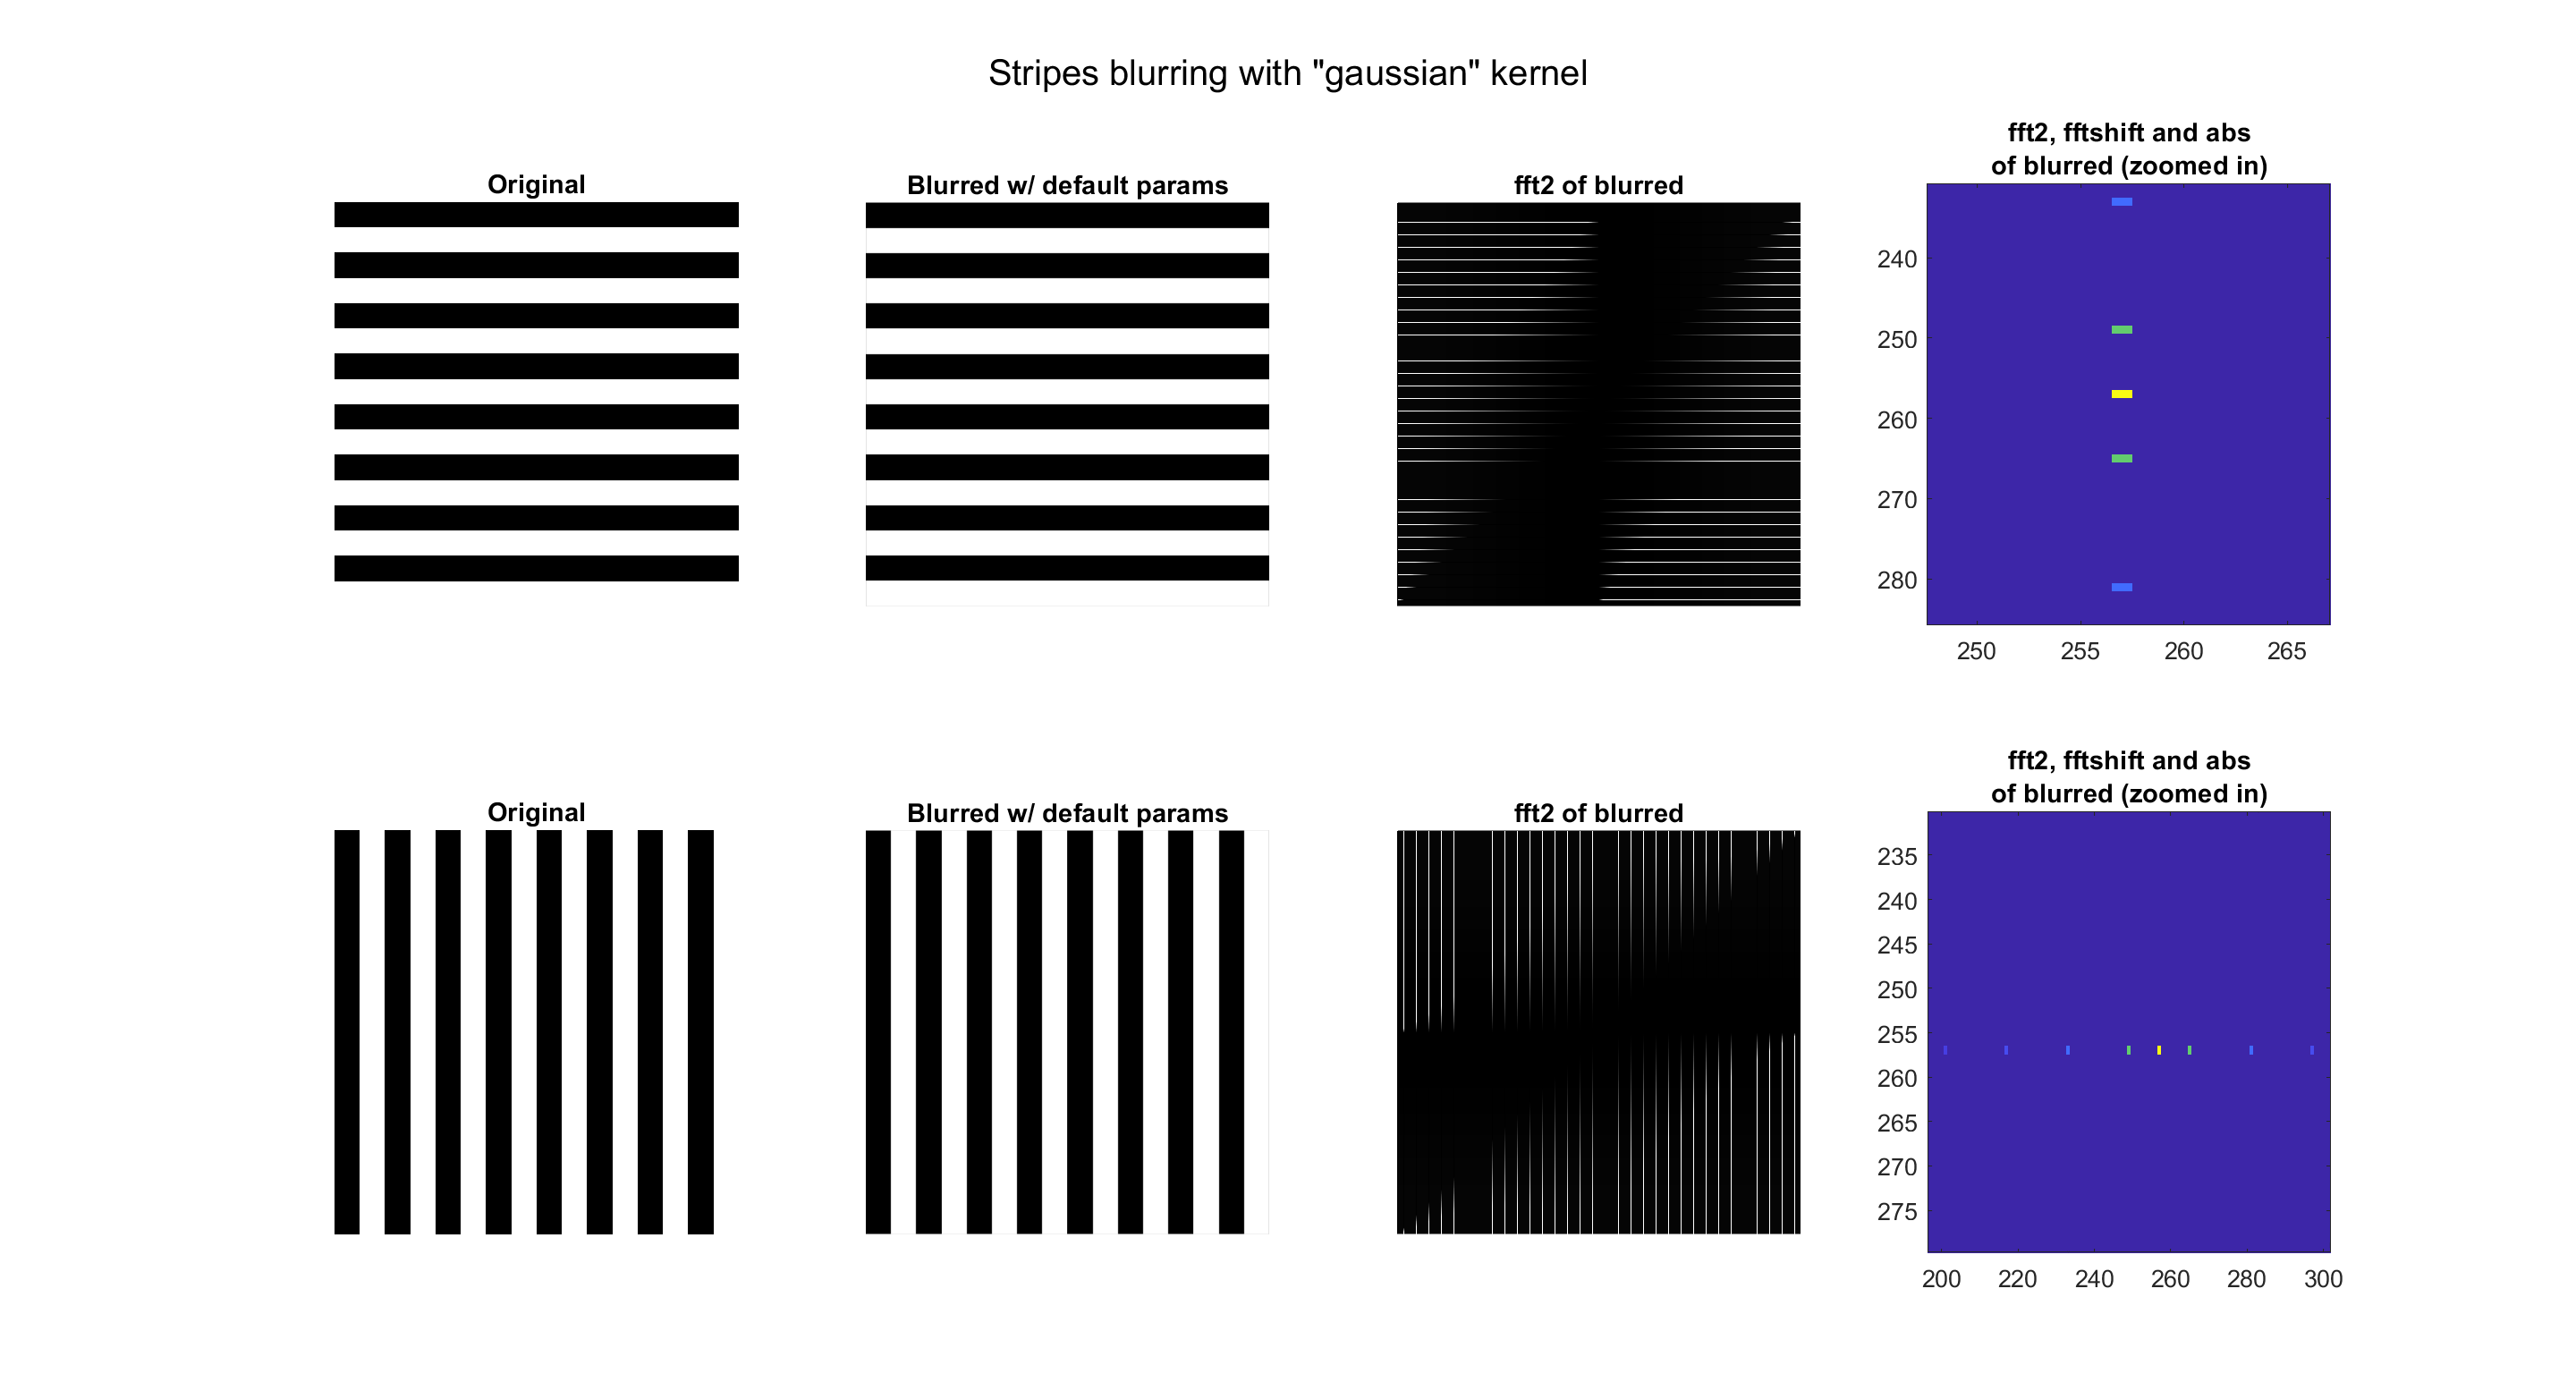
\includegraphics[width=0.75\linewidth]{Doc/Graphics/Part1/Q14b.png}
% \end{figure}

% \begin{figure}[H]
%     \centering
%     \includegraphics[width=0.75\linewidth]{Doc/Graphics/Part1/Q14c.png}
% \end{figure}

% \textbf{Rectangle and Disks:}

% Even though the images appear well blurred with the Motion kernel, the FT does not display that much information in the image, mostly being focused in the corners and the spectrum being focused sharply in the middle for the rectangle image, and in a vertical line for the circle image. Note, we had to give parameters for length and $\theta$ to get a visible result with this kernel. For the other kernels, we used the default parameters.

% The blurring of the rectangle and disk images is not quite as visible when displaying only the blurred image with the Gaussian kernel, as compared to the Motion kernel, however from the FT it is quite obvious that something has happened to the image. Particularly the circle image displays an  interesting pattern that seems to repeat throughout the image and is concentrated in the center. The Fourier spectrum in the rightmost subplot shows a similar spectrum as the horizontal stripes, however the elements continue throughout the whole spectrum (in the vertical direction) instead of being concentrated only in the middle. The Log kernel again detects the edges of the rectangle and circle, and the mathematically repeating pattern in the FT images is even stronger.

% An example of blurring and FT of the rectangle and circle images with the Gaussian kernel can be seen below.

% \begin{figure}[H]
%     \centering
%     \includegraphics[width=0.75\linewidth]{Doc/Graphics/Part1/Q14e.png}
% \end{figure}

\textbf{Question 15:}
\textit{Write a program that extracts the specific field in the image Champs.jpg (see Fig. 5).}

Since the field has periodic grooves, we can isolate it by narrowing down the range of allowable frequencies from the Fourier spectrum. We want to match the orientation of the field in the spectrum, while also blocking of values close to the origin of the spectrum, which carry noise and are too low in frequency to be relevant.

\begin{figure}[H]
    \centering
    \includegraphics[width=\textwidth]{Doc/Graphics/Part1/Part1_Question15.png}
    \label{fig:enter-label}
\end{figure}


% ~~~~~~~~~~~~~~~~~~~~~~~~~~~~~~~~
% Subsection: Deblurring
% ~~~~~~~~~~~~~~~~~~~~~~~~~~~~~~~~
\subsection{Deblurring}
In this section, we will see some examples of image deblurring algorithms through linear modelization.

The main sources of blur in an image are:
\begin{itemize}
    \item Bad focalization,
    \item Moving blur,
    \item Atmospheric turbulence,
    \item etc.
\end{itemize}

\subsubsection{Linear Modelization}

As a first approximation, a blurred image can be modelled as follows:
\begin{equation}
    Y = H  *  I + B
\end{equation}
where:
\begin{itemize}
    \item $Y$ is the blurred image to be restored,
    \item $H$ is the convolution kernel,
    \item $I$ is the original image to be estimated,
    \item $B$ is Gaussian additive noise.
\end{itemize}

\textbf{Question 16:}
\textit{Why do we have chosen this model? What are the limits of this model with respect to a single lens model?}

This model was most likely chosen because of its simplicity in explaining how noise can be modelled (and added) to an image. However, the limits of this model is that it assumes a "single lense model", i.e., that only one form of noise (the one modeled) is present in a given image. This model is not enough to describe real-life situations, as very seldom does an image only contain such noise as represented in this model. 

The model also does not account for spatially varying blur, i.e., the blur for each pixel is based on one single value present throughout the whole convolution kernel. In a real-life situation, images might be blurred quite unevenly throughout the image. objects closer to the camera lense might also be differently blurred than objects further away, however, in this image since it is taken from a great distance, that approximation might be reasonable.

The model also assumes only linear distortion effects and does not take into account nonlinear effects such as sensor saturation (certain intensities might get clipped), optical aberrations (e.g. distortion and chromatic aberration) and motion blur (objects at different speeds blur differently). The latter of which is most likely neglectable for an earth observation application such as this.

Finally, the model assumes the only present noise form would be Gaussian noise, however, many other noise forms exist in real images such as Poisson or salt-and-pepper noise.

\textit{Load the image of Toulouse (\textbf{toulouse.bmp}), blur this image with a $(2T+1)$-sized square kernel (Typically $T = 3$). The convolution kernel is thus $h(x,y) = \alpha$ if $|x| \leq T$ and $|y| \leq T$, with $\alpha = \frac{1}{(2T+1)^2}$.
}

The original image with added blur and noise can be seen in \autoref{fig:resultQ16}. The chosen parameters for the processing are $T=3$ and a standard deviation of 2 for the gaussian noise.

\begin{figure}[!ht]
    \centering
    \begin{subfigure}{0.32\textwidth}
        \centering
        \includegraphics[width=\textwidth]{Doc/Graphics/Part1/Q17_Original.png}
        \caption{Original}
    \end{subfigure}
    \hfill
    \begin{subfigure}{0.32\textwidth}
        \centering
        \includegraphics[width=\textwidth]{Doc/Graphics/Part1/Q17_Blurred.png}
        \caption{Blurred}
    \end{subfigure}
    \hfill
    \begin{subfigure}{0.32\textwidth}
        \centering
        \includegraphics[width=\textwidth]{Doc/Graphics/Part1/Q17_Noisy.png}
        \caption{Blurred and noisy}
    \end{subfigure}
    \caption{Processed images}
    \label{fig:resultQ16}
\end{figure}

% \begin{figure}[H]
%     \centering
%     \includegraphics[width=1\linewidth]{Doc/Graphics/Part1/Q16.png}
% \end{figure}



\textbf{Question 17:}
\textit{Compare the spectrums of the original image and of the blur image: what do you observe? Justify.}

We can see that the spectrum of the blurred images has a repeating pattern of squares, which decrease in intensity. This is due to the blurring kernel being essentially a box function, whose Fourier spectrum is a cardinal sine function in both axes. Once noise is added, the sharp features are washed out, and the aforementioned repeating patterns are most visible towards the axes, where the Fourier transform of the blurring kernel yielded the largest amplitudes initially.

\begin{figure}[!ht]
    \centering
    \begin{subfigure}{0.32\textwidth}
        \centering
        \includegraphics[width=\textwidth]{Doc/Graphics/Part1/Q17_FT_Spectrum_Original.png}
        \caption{Original}
    \end{subfigure}
    \hfill
    \begin{subfigure}{0.32\textwidth}
        \centering
        \includegraphics[width=\textwidth]{Doc/Graphics/Part1/Q17_FT_Spectrum_Blurred.png}
        \caption{Blurred}
    \end{subfigure}
    \hfill
    \begin{subfigure}{0.32\textwidth}
        \centering
        \includegraphics[width=\textwidth]{Doc/Graphics/Part1/Q17_FT_Spectrum_Blurred and Noisy.png}
        \caption{Blurred and noisy}
    \end{subfigure}
    \caption{Fourier Spectrum}
    \label{fig:enter-label}
\end{figure}
\FloatBarrier





% Not much can be said about the fft2 and FT spectrum for both images. In the fft2 we see a typical even random distribution of frequencies and in the abs() domain, these are concentrated to either being 1 or 0 and visible only around the zero-point of the graph when zooming in. The Log of the FT spectrum however shows quite a difference when comparing the original and blurred/noisy image, and remarkably we can see a "cross" pattern in the center of the log spectrum for the blurred/noisy image.

% The fft2, FT spectrum and log of the FT spectrum can be seen in the image below.
% Note that the FT spectrum and log FT spectrum are zoomed in for clarity.


% \begin{figure}[H]
%     \centering
%     \includegraphics[width=0.75\linewidth]{Doc/Graphics/Part1/Q17a.png}
% \end{figure}

% To further the comparison, in exaggeration the difference between the two images and their spectra is shown in the image below.
% \TODO{Any comment on this difference?}

% \begin{figure}[H]
%     \centering
%     \includegraphics[width=0.75\linewidth]{Doc/Graphics/Part1/Q17b.png}
% \end{figure}

\subsubsection{Blur Estimation}
The objective is here to estimate a posteriori the value of $T$, \textit{i.e.} from the blurred image.

\noindent In dim 1, $h(x) = \sqrt{\alpha}$ if $|x| \leq T$. The DFT is

\begin{equation}
\label{eq:DFT}
\mathcal{H}(u) = \sum_{x=-T}^{+T} h(x)e^{-j 2\pi \frac{ux}{N}} = \frac{1}{2T+1} \sum_{x=-T}^{+T} w^x
\end{equation}

However,

\[
\sum_{x=-T}^{+T} w^x = \frac{w^{-T} - w^{T+1}}{1 - w} = \frac{w^{-T-\frac{1}{2}} - w^{T+\frac{1}{2}}}{w^{-\frac{1}{2}} - w^{\frac{1}{2}}}
\]

Thus,

\begin{equation}
\label{eq:H(u)}
\mathcal{H}(u) = \frac{1}{2T+1} \frac{\sin\left(2\pi \frac{u}{N} (T + \frac{1}{2})\right)}{\sin\left(\pi \frac{u}{N}\right)}
\end{equation}

In this case, $N = 512$, $u = -512 \dots 512$. In dim 2, $h(x,y) = h(x)h(y)$.

\textbf{Question 18:}
\textit{Propose a cardinal sinus function that have the same zeros than H(u) (superpose the two functions). What conclusion could you give from these properties? Could you estimate T ?}

If we work the above \autoref{eq:H(u)} a bit we can extract from it two separate cardinal sine functions. As a reminder, $sinc(x) = \frac{sin(x)}{x}$:
\begin{equation}
\begin{split}    
    \mathcal{H} &= \frac{1}{(2T +1)} \frac{2 \pi \frac{u}{N}(T + \frac{1}{2})}{2 \pi \frac{u}{N}(T + \frac{1}{2})} \frac{\sin 2 \pi \frac{u}{N}(T + \frac{1}{2})}{\sin ( \pi \frac{u}{N})}
    \\
    &= \frac{\pi\frac{u}{N} \cancel{(2 T +1)}}{\cancel{(2T+1)}  2\pi \frac{u}{N}(T+\frac{1}{2})} 
    \frac{\sin 2 \pi \frac{u}{N}(T + \frac{1}{2})}{sin( \pi \frac{u}{N})}
    \\
    &= \frac{sinc (2 \pi \frac{u}{N}(T + \frac{1}{2}))}{sinc( \pi \frac{u}{N})}
\end{split}
\end{equation}

The zeros of this function, will be zero when the sinc function in the nominator approaches zero. This happens when the nominator of this sinc function in turn approaches zero:
\begin{equation}
\begin{split}
    &sinc (2 \pi \frac{u}{N}(T + \frac{1}{2})) = 0 \\
    & \frac{sin( 2 \pi \frac{u}{N}(T + \frac{1}{2}) )}{2 \pi \frac{u}{N}(T + \frac{1}{2})} = 0 \\
    & sin(2 \pi \frac{u}{N}(T + \frac{1}{2})) = 0
\end{split}
\end{equation}
This occurs when:
\[
2 \pi \frac{u}{N}(T + \frac{1}{2}) = k \pi, k \in \mathbb{Z}
\]
or when:
\begin{equation}
\label{eq:zeros}
u = \frac{k N}{2 (T + \frac{1}{2})}
\quad \Rightarrow \quad
T = \frac{k N}{2 u} - \frac{1}{2} 
\end{equation}

One conclusion we can draw from this is that the blur removes certain frequencies, i.e., zeros in the spectrum. This indicates a loss of information at those points. This means that blurred images lose high-frequency details making sharp edges appear smoother.

An algorithmic approach to estimate T-values would then be to first study the image and find out at what frequencies, $u$, the FT approaches zero values at the different harmonics (probably enough at $k=1$). 
Then we could based on this frequency calculate the T-value from \autoref{eq:zeros} for a known $N$ and the already identified frequency $u$. 


\textit{Compare the original image spectrum and the blurred image spectrum (using eventually the log function):}

The difference between the original image and the blurred image is as expected very pronounced in the square pattern, but also very large in the center of the spectrum.

\begin{figure}[!ht]
    \centering
    \hspace*{\fill}
    \begin{subfigure}{0.32\textwidth}
        \centering
        \includegraphics[width=\textwidth]{Doc/Graphics/Part1/Q18_FT_Spectrum.png}
        \caption{Linear scale}
    \end{subfigure}
    \hfill
    \begin{subfigure}{0.32\textwidth}
        \centering
        \includegraphics[width=\textwidth]{Doc/Graphics/Part1/Q18_FT_Spectrum_Log.png}
        \caption{Logarithmic scale}
    \end{subfigure}
    \hspace*{\fill}    
    \caption{Difference of the Fourier spectra}
    \label{fig:enter-label}
\end{figure}

\textbf{Question 19:} \textit{Estimate T.}

Because of the periodicity, we can sum the spectrum in both dimensions to smooth out the noise and contribution from the images spectrum.

\begin{figure}[!ht]
    \centering
    \hspace*{\fill}
    \begin{subfigure}{0.45\textwidth}
        \centering
        \includegraphics[width=\textwidth]{Doc/Graphics/Part1/Q19_SumX.png}
        \caption{$x$-direction}
    \end{subfigure}
    \hfill
    \begin{subfigure}{0.45\textwidth}
        \centering
        \includegraphics[width=\textwidth]{Doc/Graphics/Part1/Q19_SumY.png}
        \caption{$y$-direction}
    \end{subfigure}
    \hspace*{\fill}    
    \caption{Sum of the Fourier Spectrum in one dimension}
    \label{fig:enter-label}
\end{figure}

We can see how the oscillations due to the cardinal sine can be found in the summed up spectrum. In fact, this is due to the images spectrum being multiplied with the cardinal sine, hence the appearance being not just the cardinal sine. We can nonetheless try to estimate $T$ by fitting sinc functions whose zeros correspond to the local minima of the sums. Depending on which minimum we fit, the value we obtain is roughly $T = 2.0$ to $T = 2.7$.


% With the above described algorithmic approach we created a MatLab script to estimate the T value for the first harmonic $k=1$ and the output gives the following estimates:
% \begin{lstlisting}
%     Near-zero frequency components:
%      fx      fy 
%     ____    ____
    
%     -308    -404
%     -204    -108
    
%     Estimated T: 0.33
%     Estimated T: 0.75
%     Estimated T: 0.13
%     Estimated T: 1.87
% \end{lstlisting}

% Out of these values the last one is closest to our initial defined T value when we generated the image, however, this is not close at all to the real value. It took quite a lot of playing around with the sampling threshold to even get close to this and in the end, the noise we originally added to the blurred image might make the estimation of the T-value simply too unreliable. There might also be something wrong in the algorithm where we try to find which frequency the first harmonic 0 is approached.


\subsubsection{Image Deblurring}

Now, image deblurring (or image restoration) can be done using multiple methods. We focus on two of them:
\begin{itemize}
    \item Inverse Filtering: 
    \item Wiener Filtering: 
\end{itemize}

Let $g(x, y)$ be the inverse filter of $h(x, y)$. In the spectral domain, we have:
\begin{equation}
    G = \frac{1}{H}
\end{equation}

The estimated restored image $\hat{I}$ is:
\begin{equation}
    \hat{I} = GY = GHI + GB = I + GB
\end{equation}

The following program allows to apply this process:
\begin{lstlisting}
    SeuilMax = 11 ;
    hh = zeros(TailleImage);
    centre = [1 1] + floor(TailleImage/2) ;
    ext = (TailleFiltre-[1 1])/2;
    ligs = centre(1) + [-ext(1):ext(1)];
    cols = centre(2) + [-ext(2):ext(2)];
    
    h = ones(TailleFiltre)/prod(TailleFiltre);
    hh(ligs,cols) = h;
    hh = ifftshift(hh);
    
    H = fft2(hh);
    
    ind = find(abs(H)<(1/SeuilMax));
    H(ind) = (1/SeuilMax)*exp(j*angle(H(ind)));
    
    G = ones(size(H))./H;
    
    (...)
\end{lstlisting}


\textbf{Question 20:}
\textit{Complete this program (only 2 lines!) to process inverse filtering method.}

The full code is provided in the same source code directory in the \texttt{Restauration\_ToBeCompleted.m} file. 
The two lines to complete this program (with some small other adjustments) can be seen in the \textit{Restauration.m} file in this directory on lines 106 and 107 -- and below:
\begin{lstlisting}
    TFdIrest = G.*TFdIf;
    Irest = real(ifft2(TFdIrest));
\end{lstlisting}


\textbf{Question 21:}
\textit{What’s happen with the image marcheur.jpg ?}

We can see that the motion blurred, but non-noisy \texttt{marcheur.jpg} picture is reconstructed partially, but not particularly well. The situation is the same also when noise is added. We can see that the algorithm performs significantly better for the \texttt{toulouse.bmp} image. This is because the inverse filtering method here only applies the reverse operation to blurring with a square kernel. Since the motion blur kernel is not square, this method doesn't work on the \texttt{marcheur.jpg} image.  

\begin{figure}[H]
    \centering
    \includegraphics[width=\linewidth]{Doc/Graphics/Part1/Q21a.png}
\end{figure}

\begin{figure}[H]
    \centering
    \includegraphics[width=1\linewidth]{Doc/Graphics/Part1/Q21b.png}
\end{figure}

